%% Copernicus Publications Manuscript Preparation Template for LaTeX Submissions
%% ---------------------------------
%% This template should be used for copernicus.cls
%% The class file and some style files are bundled in the Copernicus Latex Package, which can be downloaded from the different journal webpages.
%% For further assistance please contact Copernicus Publications at: production@copernicus.org
%% https://publications.copernicus.org/for_authors/manuscript_preparation.html


%% Please use the following documentclass and journal abbreviations for discussion papers and final revised papers.

%% 2-column papers and discussion papers
\documentclass[journal abbreviation, manuscript]{copernicus}



%% Journal abbreviations (please use the same for discussion papers and final revised papers)


% Advances in Geosciences (adgeo)
% Advances in Radio Science (ars)
% Advances in Science and Research (asr)
% Advances in Statistical Climatology, Meteorology and Oceanography (ascmo)
% Annales Geophysicae (angeo)
% Archives Animal Breeding (aab)
% ASTRA Proceedings (ap)
% Atmospheric Chemistry and Physics (acp)
% Atmospheric Measurement Techniques (amt)
% Biogeosciences (bg)
% Climate of the Past (cp)
% DEUQUA Special Publications (deuquasp)
% Drinking Water Engineering and Science (dwes)
% Earth Surface Dynamics (esurf)
% Earth System Dynamics (esd)
% Earth System Science Data (essd)
% E&G Quaternary Science Journal (egqsj)
% Fossil Record (fr)
% Geochronology (gchron)
% Geographica Helvetica (gh)
% Geoscience Communication (gc)
% Geoscientific Instrumentation, Methods and Data Systems (gi)
% Geoscientific Model Development (gmd)
% History of Geo- and Space Sciences (hgss)
% Hydrology and Earth System Sciences (hess)
% Journal of Micropalaeontology (jm)
% Journal of Sensors and Sensor Systems (jsss)
% Mechanical Sciences (ms)
% Natural Hazards and Earth System Sciences (nhess)
% Nonlinear Processes in Geophysics (npg)
% Ocean Science (os)
% Primate Biology (pb)
% Proceedings of the International Association of Hydrological Sciences (piahs)
% Scientific Drilling (sd)
% SOIL (soil)
% Solid Earth (se)
% The Cryosphere (tc)
% Web Ecology (we)
% Wind Energy Science (wes)


%% \usepackage commands included in the copernicus.cls:
%\usepackage[german, english]{babel}
%\usepackage{tabularx}
%\usepackage{cancel}
%\usepackage{multirow}
%\usepackage{supertabular}
%\usepackage{algorithmic}
%\usepackage{algorithm}
%\usepackage{amsthm}
%\usepackage{float}
%\usepackage{subfig}
%\usepackage{rotating}


\begin{document}

\title{Synergistic radar and radiometer retrievals of ice clouds}

% \Author[affil]{given_name}{surname}

\Author[1]{Simon}{Pfreundschuh}
\Author[1]{Patrick}{Eriksson}
\Author[2]{Stefan A.}{Buehler}
\Author[2]{Manfred}{Brath}
\Author[4]{David}{Duncan}
\Author[3]{Richard}{Larsson}
\Author[2]{Robin}{Ekelund}

\affil[1]{Department of Space, Earth and Environment, Chalmers University of Technology, 41296 Gothenburg, Sweden}
\affil[2]{Meteorologisches Institut, Fachbereich Geowissenschaften, Centrum für Erdsystem und Nachhaltigkeitsforschung (CEN), Universität Hamburg, Bundesstraße 55, 20146 Hamburg, Germany}
\affil[3]{Max Planck Institute for Solar System Research, Justus-von-Liebig-Weg 3, 37077 Göttingen, Germany}
\affil[4]{ECMWF, Shinfield Park, Reading RG2 9AX, United Kingdom}
%% The [] brackets identify the author with the corresponding affiliation. 1, 2, 3, etc. should be inserted.

\runningtitle{Retrieving frozen hydrometeors from combined radar and sub-millimter observations}
\runningauthor{Simon Pfreundschuh}
\correspondence{Simon Pfreundschuh (simon.pfreundschuh@chalmers.se)}

\received{}
\pubdiscuss{} %% only important for two-stage journals
\revised{}
\accepted{}
\published{}

%% These dates will be inserted by Copernicus Publications during the typesetting process.

\firstpage{1}

\maketitle

\begin{abstract}
  The upcoming Ice Cloud Imager (ICI) radiometer, to be launched on board the
  second generation of European operational meteorological satellites
  (Metop-SG), will be the first microwave imager to provide sub-millimeter
  observations of the atmosphere. The Microwave Imager (MWI) radiometer will be
  flown on the same satellites and complement the ICI sensor with observations
  at traditional millimeter wavelengths. With the aim of maximizing the
  scientific turnout from Metop-SG program, this study explores the potential of
  combining the observations from the MWI and ICI radiometers with a $94
  \ \unit{GHz}$ cloud radar for the retrieval of ice hydrometeors. Starting from
  a simplified numerical experiment, it is shown that the complementary
  information content in the radar and radiometer observations can help to
  better constrain the particle size distribution of ice particles in clouds.
  The feasibility of the combined retrieval is demonstrated by applying a
  one-dimensional, variational cloud-retrieval algorithm to simulated
  observations from a high-resolution atmospheric model. Comparison of the
  results with passive- and radar-only versions of the retrieval algorithm
  confirms that the synergistic information content from the active and passive
  observations improves the retrieval of microphysical properties of frozen
  hydrometeors. The effect of the assumed ice particle shape on the retrieval
  results is analyzed and the assumed shape is found to be crucial for obtaining
  good retrieval performance. Furthermore, the synergistic retrieval is found to be able to
  detect and retrieve supercooled clouds. The results of this study clearly
  demonstrates the potential of combined radar and radiometer observations to
  better constrain microphysical properties and improve the retrievals of
  ice hydrometeors. Such combined retrievals could thus help to reduce the
  large uncertainties in the observational record of ice in the atmosphere.
\end{abstract}


\introduction  %% \introduction[modified heading if necessary]

Ice clouds play an important role in many weather- and climate-related processes
in the atmosphere. They interact with incoming and outgoing radiation and thus
influence the Earth's energy budget. Moreover, as part of the global
hydrological cycle and due to their relation to the dynamics of the atmosphere
\citep{bony15}, observations of ice clouds provide important information to
constrain the state of the atmosphere in numerical weather prediction models
\citep{geer} as well as to validate predictions from climate models
\citep{waliser09}.

Despite the importance of observations of ice clouds for climate and weather
prediction, today's global observing system cannot provide accurate information
on the global distribution of ice in the atmosphere
\citep{eliasson11,duncan18a}. The main difficulty in sensing atmospheric ice
from space is the large variability of sizes and concentrations in which ice
particles occur in the atmosphere. The wide spectrum of ice crystal sizes, that
ranges from micro- to millimeter scales, can only be partially resolved by
currently available space-borne sensors.

The sensitivity of a remote sensing system to ice particles of a given size is
determined mainly by its observing frequencies. The scattering of radiation by
ice particles is strongest for sizes roughly equal to the wavelength, $\lambda$,
of the radiation. For particles with sizes much smaller than $\lambda$, the
sensitivity decreases rapidly, making them practically invisible to the sensor.
Although the strength of the interaction between particles and radiation
decreases as the wavelength becomes much larger than the particle size, it
remains strong enough for the cloud signal to saturate in the presence of
thicker clouds, leading to loss of sensitivity further down the line of sight.

The observing frequencies that are currently available for measuring ice from
space are limited to the microwave, infrared and optical domain. Infrared and
optical sensors provide sensitivity to small ice particles but cannot sense
significant parts of the ice mass of thicker clouds due to saturation of the
signal. Microwave observations, in contrast, provide sensitivity throughout the
whole atmospheric column but are insensitive to small ice particles. Although
radars and lidars generally provide greater sensitivity than their passive
counterparts, they are ultimately limited by the same principles.

To narrow the size-sensitivity gap between the infrared and traditional microwave
sensors, the upcoming Ice Cloud Imager (ICI) will extend the microwave
frequencies available for studying clouds with channels at $243$, $325$, $448$ and
$664\ \unit{GHz}$. This extension of the smallest currently available microwave
wavelength from $1.6\ \unit{mm}$ at $183\ \unit{GHz}$ down to the sub-millimeter
domain ($0.45\ \unit{mm}$ at $664\ \unit{GHz}$) will significantly improve the
size-sensitivity of space-borne microwave observations of clouds.

Together with ICI, also the newly developed Microwave Imager (MWI), will be
flown on the satellites of the Metop-SG program. MWI will complement ICI's
observations with measurements at traditional millimeter wavelengths. MWI's
channels, that cover the frequency range from $19\ \unit{GHz}$ up to
$183\ \unit{GHz}$, will provide additional sensitivity to liquid and frozen
precipitation and water vapor.

The advent of space-borne sub-millimeter radiometry of clouds brings with it
great potential for the study ice in the atmosphere. The information content and
retrieval performance from radiometer observations alone has been studied in
detail for column-integrated ice mass \citep{jimenez07, wang17, brath18a} as
well as for the vertical distribution of ice in the atmosphere \citep{birman17, grutzun18,
  aires19}. Also the concept of combining millimeter and sub-millimeter
radiometer observations with active observations from a cloud radar has been
investigated \citep{evans05, jiang19}.

This work applies the concept of combined radiometer and radar retrievals to the
upcoming ICI and MWI sensors combined with a conceptual W-band cloud radar and
explores its potential for retrieving vertically-resolved distributions of
frozen hydrometeors in the atmospheric column. The particular objective of this
study is to explore the fundamental synergies between radar and passive
sub-millimeter observations. It aims to investigate the extent to which the
combined active and passive observations can constrain the microphysics of ice
particles in the atmosphere. Starting from a simplified numerical experiment,
the complementarity of the information content of the active and passive
observations is demonstrated. In addition to this, simulated results from a
synergistic, variational cloud-retrieval algorithm are presented. The algorithm
is applied to synthetic observations of cloud scenes from a high-resolution
atmospheric model and used to further explore the synergies between the active
and passive observations.

The presented research has been conducted as part of a larger study funded by
the European Space Agency, which aimed to evaluate the concept of a future radar
mission to fly in constellation with ICI on board the satellites of the Metop-SG
program. Inspired by the success of the Global Precipitation Measurement (GPM,
\cite{hou14}) mission, the approach of this tentative mission is to perform
vertically-resolved, high-accuracy retrievals of hydrometeors from the
co-located active and passive observations at the swath center of the passive
imager. The combined retrieval results are then used to constrain passive-only
profile retrievals with the aim of extending the profiling capabilities of the
radar to the wide swath of the passive imager.

Following this introduction, Section \ref{sec:methods_and_data} introduces the
test data, sensor configuration and the developed retrieval algorithm on which
the study is based. This is followed by the experimental results on the
information content of the combined observations and the retrieval results of
the joint retrieval on selected test scenes in Section \ref{sec:results}. The
article closes with a discussion of the results in Section \ref{sec:discussion}
and conclusions in section \ref{sec:conclusions}.


\section{Methods and data}
\label{sec:methods_and_data}

The synergistic retrieval is tested using simulated observations of cloud scenes
from a high-resolution atmospheric circulation model. This section presents the
selected reference cloud scenes, sensor configuration and basic modeling
assumptions used in the radiative transfer simulations. In addition to this, the
theoretical formulation of the combined cloud-retrieval algorithm is introduced.

\subsection{Reference cloud scenes}

The cloud scenes that are used to generate the synthetic cloud observations are
taken from the Global Environmental Multiscale Model (GEM, \cite{cote98}). For
this study, we restrict ourselves to two designated, two-dimensional test
scenes, that are displayed in Fig.~\ref{fig:overview}. The test scenes have a
horizontal resolution of $1\ \unit{km}$ and both extend over $800\ \unit{km}$.
The scenes were chosen with the aim of covering a large range of cloud
structures and compositions so as to ensure a realistic assessment of the
retrieval. The first test scene, shown in panel (a), is located in the tropical
Pacific and contains a convective storm system in the right half of the scene
and its anvil that extends into the left half of the scene. The second scene,
shown in panel (b), is located in the North Atlantic and contains an  ice
cloud in the first quarter and a low-level, mixed-phase cloud in the remainder
of the scene.

\begin{figure}[h!]
\centering
\includegraphics[width = 0.8\textwidth]{figures/fig01.png}
\caption{The distribution of total hydrometeor mass content in the two
cloud scenes used to test the retrieval. Colored lines show the
 $m = 10^{-5}\  \unit{kg/m^3}$ contour for different
 hydrometeor species.}
\label{fig:overview}
\end{figure}


The GEM model, from which the scenes are taken, uses six types of hydrometeors
to represent clouds and precipitation \citep{milbrandtyau05}: Two classes of
liquid hydrometeors (rain and liquid cloud) and four of frozen hydrometeors
(cloud ice, snow, hail and graupel). The particle size distribution (PSD) of
each hydrometeor type is parametrized by its particle number concentration and
mass density. The full particle size distribution can be prognosed from the two
moments using a species-dependent parametrization and mass-size relationship.
The parameters of the mass-size relationship are given in
Tab.~\ref{tab:species_parameters}. As shown in the table, the densities of all
hydrometeor species in the model are assumed to scale with a power of three,
which leads to unrealistically high densities for large particles.

\begin{table}
  \centering
  \caption{Particle-model names, IDs and parameters $\alpha, \beta$ of the
    mass-size relationships $m = \alpha D_\text{max}^\beta$, where
    $D_\text{max}$ is the maximum diameter of the particle. The ID column
    contains the particle shape identifier of the particle model in the
    \citet{eriksson18} scattering database.}
  \label{tab:species_parameters}
  \begin{tabular}{l|c|c|c|c}
    Hydrometeor species & Particle shape & ID & $\alpha$ & $\beta$ \\
    \hline
    Cloud ice    & GemCloudIce  & 31 & 440   & 3 \\
    Snow         & GemSnow      & 32 & 52.4  & 3 \\
    Graupel      & GemGraupel   & 33 & 209.4 & 3 \\
    Hail         & GemHail      & 34 & 471.2 & 3 \\
    Rain         & LiquidSphere & 25 & 523.6 & 3 \\
    Liquid cloud & LiquidSphere & 25 & 523.6 & 3 \\
  \end{tabular}
\end{table}

Examples of particle size distributions of frozen hydrometeors are displayed in
Fig.~\ref{fig:gem_psds}. The four panels display the prognosed particle size
distributions for the four frozen hydrometeor types together with renderings of
the particle shapes used in the forward simulations. As these plots show, the
assumed particle size distributions across different ice species vary mostly in
their horizontal and vertical scaling, whereas the function shape shows less
variability. Furthermore, an important characteristic of the model can be
identified here, that will help to better understand the retrieval results
presented later: Cloud ice in the model is characterized by high particle number
densities and small particle sizes, whereas snow exhibits lower number
concentrations and larger particles.


\begin{figure}[h!]
\centering \includegraphics[width = \textwidth]{figures/fig02.png}
\caption{Realizations of particle size distributions from the cloud scenes used
  in this study. The number particle density is plotted with respect to the
  volume-equivalent diameter $D_\text{eq}$. Shown are the PSDs corresponding to
  100 randomly chosen grid points with a mass concentration higher than
  $10^{-6}\ \unit{kg/m^3}$. Line color encodes the corresponding mass density.}
\label{fig:gem_psds}
\end{figure}


\subsection{Simulated cloud observations}

A simulated observation is generated for each vertical profile in the
model test scenes. The simulations apply the same microphysics scheme
as the model, meaning that they use the same six hydrometeor classes
and PSD parametrizations.

\subsubsection{Sensor configuration}
\label{sec:sensors}

Simulations of observed passive brightness temperatures are performed for the 11
highest-frequency channels of the MWI radiometer and all channels of the ICI
radiometer. The passive observations are combined with a W-band cloud radar
similar to the CloudSat Cloud Profiling Radar (CPR)
\citep{stephens02,tanelli08}. The choice of a CPR-type radar is based mainly on
the success and longevity of the CloudSat mission, that clearly demonstrates the
maturity and robustness of the technology.

A number of simplifications are applied for the generation of the synthetic
cloud observations: Firstly, the beams of all three sensors are modeled as
perfectly coincident pencil beams. Secondly, a synthetic observation is
generated for each vertical profile from the model scenes by simulating a
one-dimensional, plane-parallel atmosphere, the properties of which are taken
from the corresponding model profile. It follows from these modeling decisions
that the atmosphere is assumed to be homogeneous across the beams of the active
and passive sensors and that they all sense the same atmospheric volume. For
space-borne observations, this would certainly not be the case and will incur a
forward modeling error that is not accounted for in this study. Since the
 focus of this study are the fundamental synergies between the active and passive
 observations, quantifying the impact of beam width and inhomogeneity is left
 for future investigation.

Observations from the ICI radiometer are simulated by performing a single,
non-polarized radiative transfer simulation located at the centers of the pass
bands of each channel and averaging the resulting brightness temperatures. For
channels with multiple polarizations, only a single simulation is performed.
To compensate for this, the noise of the corresponding channel is reduced by a
factor of $\sqrt{2}$. The simulated ICI channels and assumed noise levels are
presented in  Tab.~\ref{tab:channels}. The off-nadir viewing angle of ICI
is assumed to be $48\unit{^\circ}$ at the sensor.

Observations from the MWI radiometer are simulated in a similar manner as those
from ICI. However, from MWI only channels with frequencies larger than or equal
to $89\ \unit{GHz}$ are used. The reason for this is that the footprints of the
channels with frequencies lower than $89\ \unit{GHz}$ have full-width at half
maximum of $50\ \unit{km}$ compared to only $10\ \unit{km}$ for the
higher-frequency channels. Due to the very small overlap of the footprints of
these low-frequency channels with that of the radar, it is assumed they would
not be beneficial for a synergistic retrieval and are therefore disregarded
here. The included MWI channels are listed in Tab.~\ref{tab:channels}.

\begin{table}[hbpt]
\caption{Channels of the MWI and ICI radiometers used in the retrieval.}
\label{tab:channels}
    \begin{tabular}{c|r|r}
    \multicolumn{3}{c}{MWI}\\
    Channel & Freq. [GHz] & Noise [K]\\
    \hline
    MWI-8  & $89$              & $1.1$ \\
    MWI-9  & $118.75 \pm 3.2$  & $1.3$ \\
    MWI-10 & $\pm 2.1$         & $1.3$ \\
    MWI-11 & $\pm 1.4$         & $1.3$ \\
    MWI-12 & $\pm 1.2$         & $1.3$ \\
    MWI-13 & $165.5 \pm 0.75$  & $1.3$ \\
    MWI-14 & $183.31 \pm 7.0$  & $1.2$ \\
    MWI-15 & $ \pm 6.1$        & $1.2$ \\
    MWI-16 & $ \pm 4.9$        & $1.2$ \\
    MWI-17 & $ \pm 3.4$        & $1.2$ \\
    MWI-18 & $ \pm 2.0$        & $1.3$ \\
    \end{tabular}%
    \hspace{1cm}%
    \begin{tabular}{c|r|r}
    \multicolumn{3}{c}{ICI}\\
    Channel & Freq. [GHz] & Noise [K] \\
    \hline
    ICI-1  & $183.31 \pm 7.0$ & $0.8$\\
    ICI-2  & $       \pm 3.4$ & $0.8$\\
    ICI-3  & $       \pm 2.0$ & $0.8$\\
    ICI-4  & $243    \pm 2.5$ & $\frac{1}{\sqrt{2}} \cdot 0.7$\\
    ICI-5  & $325.15 \pm 9.5$ & $1.2$\\
    ICI-6  & $       \pm 3.5$ & $1.3$\\
    ICI-7  & $       \pm 1.5$ & $1.5$\\
    ICI-8  & $448    \pm 7.2$ & $1.4$\\
    ICI-9  & $       \pm 3.0$ & $1.6$\\
    ICI-10 & $       \pm 1.4$ & $2.0$\\
    ICI-11 & $664    \pm 4.2$ & $\frac{1}{\sqrt{2}} \cdot 1.6$\\
    \end{tabular}
\end{table}

The frequency of the the cloud radar is chosen to be $94\ \unit{GHz}$ similar to
CloudSat CPR. The vertical resolution of the radar observations is assumed to be
$500\ \unit{m}$ ranging from $0.5$ to $20\ \unit{km}$ in altitude. The minimum
sensitivity is set to be $-30\ \unit{dBZ}$ and the noise at each range gate is
modeled to be independent with standard deviation $0.5\ \unit{dBZ}$. As mentioned
above, the same incidence angle as for the passive radiometers is assumed also
for the radar. In practice, this could be achieved by remapping the radar
observations to the lines of sights of the passive beams.

\subsubsection{Radiative transfer simulations}
\label{sec:orge741b86}

All simulations presented in this study were performed using Version 2.3.1245 of
the Atmospheric Radiative Transfer Simulator (ARTS, \cite{arts18}). Radar
reflectivities are computed using the ARTS' built-in single-scattering radar
solver. For the simulation of passive radiances, a hybrid solver is used that
combines the DISORT \citep{disort00} scattering solver with the ARTS standard
scheme for pencil beam radiative transfer. The hybrid solver has been added to
ARTS specifically for this study and provides approximate, analytical Jacobians,
which are required for the variational retrievals of hydrometeors. All
simulations are performed assuming an ocean surface with emissivities calculated
using the Tool to Estimate Sea‐Surface Emissivity from Microwaves to
sub‐Millimeter waves (TESSEM, \cite{prigent16}). Polarization is neglected in
all simulations performed in this study. Particle scattering data are taken from
the ARTS scattering data base (hereafter ARTS SSDB, \citet{eriksson18}). Gaseous
absorption from $N_2$, $O_2$, and $H_2O$ is modeled using the absorption models
from \cite{rosenkranz98}, ..., and ..., respectively.


\subsection{Retrieval algorithm}
\label{sec:orgb528563}

A one-dimensional, variational cloud retrieval algorithm is proposed to
retrieve distributions of frozen hydrometeors from the combined active and
passive observations. The algorithm uses the optimal estimation method (OEM)
developed by \cite{rodgers00}. The retrieved state $\mathbf{x} \in
   \mathbb{R}^n$ is determined by fitting a forward model $\mathbf{F} : \mathbb{R}^n
   \rightarrow \mathbb{R}^m$ to a set of observations $\mathbf{y} \in
   \mathbb{R}^m$. The best fit is determined by minimizing a cost function of
the form
\begin{align}
l(\mathbf{x}, \mathbf{y}) \propto
 \left(\mathbf{F}(\mathbf{x}) - \mathbf{y} \right )^T
  \mathbf{S}_e^{-1} 
  \left ( \mathbf{F}(\mathbf{x}) - \mathbf{y} \right)
+ \left ( \mathbf{x} - \mathbf{x}_a \right )^T
 \mathbf{S}^{-1}_a 
 \left ( \mathbf{x} - \mathbf{x}_a \right ).
\end{align}
%
The cost function $l(\mathbf{x}, \mathbf{y})$ corresponds to the negative
log-likelihood of the a posteriori distribution of the state $\mathbf{x}$ under
the assumptions of Gaussian a priori distribution with mean $\mathbf{x}_a$ and
covariance matrix $\mathbf{S}_a$ as well as zero-mean Gaussian measurement error
with covariance matrix $\mathbf{S}_e$.

Following Chapter~12 in \cite{rodgers00}, the quality of the retrieved state\
$\hat{\mathbf{x}}$ and corresponding fitted observations $\hat{\mathbf{y}}$ can
be assessed using 
%
\begin{align}
  \chi^2 &= (\mathbf{y} - \hat{\mathbf{y}})^T \left (
  \mathbf{S}_e (\mathbf{K}\mathbf{S}_a\mathbf{K}^T + \mathbf{S}_e)^{-1}) \mathbf{S}_e
  \right )^{-1} (\mathbf{y} - \hat{\mathbf{y}}).
\end{align}
%
Given the underlying assumptions of Gaussian measurement error and a priori,
the quantity $\chi^2$ follows a chi-square distribution with $m$ degrees of
freedom. If the retrieval produces high  $\chi^2$ values, than this is an indicator
of convergence problems or inability of the forward model to fit the observations.

\subsubsection{Measurement space}
\label{sec:orge7dc286}

The input for the retrieval algorithm is the combined observation vector
$\mathbf{y}$ consisting of the concatenated single-instrument observation
vectors from the cloud radar and the two radiometers. Measurement errors are
assumed to be independent and Gaussian distributed with standard deviations
according to the noise characteristics given in Section \ref{sec:sensors}.

\subsubsection{State space}
\label{sec:orgae5ee4e}

The proposed retrieval solves for distributions of one frozen and one liquid
hydrometeor species in the atmospheric column together with profiles of
atmospheric humidity and liquid-cloud mass density. The retrieval uses the same
vertical grid as the model scenes, which have a vertical resolution of about
$500\ \unit{m}$ throughout the troposphere. If not specified otherwise,
retrieval quantities are retrieved at this resolution.

Distributions of hydrometeors in the atmospheric column are represented using
the normalized particle size distribution formalism proposed by
\cite{delanoe05}. The PSD of a hydrometeor species at a given height level is
represented by a vertical and a horizontal scaling parameter, the mass-weighted
mean diameter $D_m$ and the normalized number density $N_0^*$. Alternative PSD
parametrizations using mass density and $D_m$ or the mass density and $N_0^*$
have been tested but no considerable effect on retrieval performance has been
observed.

The retrieval computes profiles of the two scaling parameters $D_m$ and $N_0^*$
for each of the two hydrometeor species. For each species, the shape of the PSD
described by the parameters $\alpha$ and $\beta$ is assumed fixed. The principle
is illustrated in Fig.~\ref{fig:psds_retrieval}. The plot displays the
a-priori-assumed shapes of the particle size distribution of frozen and liquid
hydrometeors. The retrieved horizontal and vertical scaling parameters, $D_m$
and $N_0^*$, are used as units for the axes of the plot so that the shape of the
PSD becomes independent of the retrieved mass density and number concentration.
For frozen hydrometeors, the values of the shape parameters $\alpha$ and $\beta$
are chosen identical to version 3 of the DARDAR-CLOUD product
\citep{cazenave18}. For liquid hydrometeors, the shape parameters are chosen so
that they are equivalent to the shape used by the GEM model for rain drops. All
calculations involving particles size distributions use the volume-equivalent
diameter $D_\text{eq}$ as size variable.

\begin{figure}
\centering
\includegraphics[width = 0.5\linewidth]{figures/fig03}
\caption{PSD parametrizations for frozen and liquid hydrometeors
 used in the cloud retrieval.}
\label{fig:psds_retrieval}
\end{figure}

The temperature-dependent a priori profile for $N_0^*$ of frozen
hydrometeors is determined using the relation from \cite{delanoe14}
%
\begin{align}
N_0^* &= \exp \left ( -0.076586 \cdot (T - 272.5) + 17.948 \right ),
\end{align}
%
where $T$ is in $\unit{K}$. The a priori profile for $D_m$ for frozen
hydrometeors is chosen so that the a priori mass density is equal to
$10^{-6}\ \unit{kg/m^3}$. For liquid hydrometeors, a fixed value for $N_0^*$ of
$10^6\ \unit{m^4}$ is assumed and the a priori profile for $D_m$ is determined
similarly as for frozen hydrometeors. Values of the mass-weighted mean diameter
$D_m$ for both hydrometeor species are retrieved in linear space, whereas the
normalized number concentration parameter $N_0^*$ is retrieved in
$\text{log}_{10}$ space. As additional constraints, the retrieval of frozen
hydrometeors is restricted to the region between the freezing layer and the
tropopause, whereas the retrieval of liquid hydrometeors is restricted to below
the freezing layer.

To further regularize the retrieval, $N_0^*$ for ice is retrieved at only
10 equally-spaced grid points between freezing layer and the tropopause.
Similarly, $D_m$  and $N_0^*$ for rain are retrieved at 10 and 4 points
between the freezing layer. This was necessary to avoid the occurrence
of runaway situations where the retrieval would falsely produce high-frequency
oscillations with unrealistically high values of $N_0^*$. An approach similar
to this one is also taken in the GPM combined precipitation retrievals
\citep{grecu16}.

Humidity in the atmospheric column is retrieved in units of relative humidity at
a vertical resolution of $1\ \unit{km}$. However, instead of retrieving relative
humidity directly, an inverse hyperbolic tangens transformation is applied to
the relative humidity profile $\mathbf{\phi}$:
%
\begin{align}
x = \text{arctanh}(\frac{2 \mathbf{\phi}}{1.1} - 1.0)
\end{align}
%
The transformation restricts the retrieved relative humidity values to
the range of $[0.0, 1.1]$. The a priori profile for relative humidity
is arbitralily chosen as
%
\begin{align}
\phi(t) = \begin{cases}
 0.7 &, 270\ \unit{K} < t \\
 0.7 - 0.01 \cdot (t - 270) & ,220 < t \leq  270\ \unit{K} \\
 0.2 \cdot (t - 270) & ,t < 220 \\
 \end{cases}.
\end{align}
%
The retrieval of liquid cloud mass density is performed at seven equally spaced
altitude level between the surface and the $230\ \unit{K}$ isotherm. In contrast
to the frozen and liquid hydrometeors, cloud water is modeled in the retrieval
forward model to be purely absorbing using the absorption model by
\cite{liebe92} for suspended liquid cloud droplets. Liquid cloud mass density is
retrieved in $\text{log}_{10}$-space and the a priori profile is set to a fixed
value of $10^{-5}\ \unit{kg / m^3}$ in the permitted region of the atmosphere.

The a priori distributions of the 6 retrieval quantities ($N_0^*$ and $D_m$ for
frozen and liquid hydrometeors, relative humidity $\phi$, cloud water) are
assumed to be independent so that the overall a priori covariance matrix
$\mathbf{S}_a$ has block-diagonal structure. Within each block, vertical
correlations between the values of a given retrieval quantity at different
altitudes are assumed to be exponentially decaying. Hence, the correlation of
the values of retrieval quantity $q$ at points $i$ and $j$ of the retrieval grid
is computed as
%
\begin{align}
\left ( \mathbf{S}_{a,q} \right )_{i, j} &= \sigma_{q,i} \sigma_{q,j}
 \cdot \exp  \left ( -\frac{d(i, j)}{l_q} \right ),
\end{align}
%
where $\sigma_{q, i}$ is the a priori uncertainty assumed for retrieval
quantity $q$ at grid point $i$, $d(i, j)$ the distance between the grid
points and $l_q$ the quantity-specific correlation length. The assumed
a priori uncertainties and correlation lengths for the retrieval quantities
are summarized in Tab.~\ref{tab:a_priori}.

\begin{table}[h!]
\caption{A priori uncertainties and correlation
 lengths used in the retrieval.}
 \centering
\label{tab:a_priori}
    \begin{tabular}{c|r|r}
     Quantity $q$ & $\sigma_q$ & $l_q$ [km]\\
    \hline
    $\log_{10}(N_{0, \text{frozen}}^*)$    & $2$                       & $2$ \\
    $D_{m, \text{ice}}$               & $300\ \unit{\mu m}$ & $2$ \\
    $\log_{10}(N_{0, \text{liquid}}^*)$    & $2                      $ & $2$ \\
    $D_{m, \text{liquid}}$            & $500\ \unit{\mu m}$ & $2$ \\
    $\text{arctanh}(\frac{2 \cdot \phi}{1.1} - 1.0)$ & $2$                       & $2$ \\
    $\log_{10}(m_\text{liquid cloud}) $ & $1$                       & $2$ \\
    \end{tabular}
\end{table}

As baselines for the assessment of the combined retrieval, also a radar-only and
a passive only-retrieval are performed. The radar-only retrieval uses the same
implementation as the combined retrieval, but only retrieves frozen and liquid
hydrometeors. For the radar-only retrieval, perfect knowledge of the atmospheric
humidity profile is assumed but liquid cloud is ignored in the retrieval forward
model.

The setup and retrieval quantities of the passive-only retrieval are similar to
the combined retrieval, with the only difference being that frozen and liquid
hydrometeors are retrieved at reduced resolution. For ice, $N_0^*$ is retrieved
at two equally spaced grid points between $0\ \unit{^\circ C}$-isotherm and
troposphere, while $D_m$ is retrieved at six. For liquid hydormeteors, the
retrieval grids for $N_0^*$ and $D_m$ are reduced to two equally spaced points
between surface and $0\ \unit{^\circ C}$-isotherm. Relative humidity is retrieved
at eleven grid points between surface and tropopause.

\section{Results}
\label{sec:results}

In the first part of this section results of a numerical experiment are
presented that investigates the complementary information content of the active
and passive observations. The remainder of this section presents the retrieval
results of the combined and the baseline retrievals applied to the reference
cloud scenes.

\subsection{Complementary information content}
\label{sec:orgdc1b0b8}

A fundamental question regarding the benefit of combining two remote sensing
observations in a retrieval is to what extent the observations contain
non-redundant information. The degree of non-redundancy in the combined
observations is what is referred to here as complementary information content.
In order to explore this complementary information content in the radar and
radiometer observations, an idealized, homogeneous cloud layer with a thickness of
$4\ \unit{km}$ located at an altitude of $10\ \unit{km}$ in a tropical atmosphere is
considered. The cloud is assumed to consist of a single frozen hydrometeor
species using the same PSD parametrization as the frozen hydrometeors used in
the cloud retrieval. As particle model, the 8-ColumnAggregate (ID 8) from the ARTS
SSDB is used.

The question that we aim to address here is whether the combination of active
and passive observations is able to constrain both the horizontal and the
vertical scaling factors of the PSD of the ice particles in the cloud. To
investigate this, the $N_0^*$ and $D_m$ parameters of the homogeneous cloud
layer are varied and observations of the cloud layer are simulated. Figure
\ref{fig:contours} displays the simulated cloud signal, i.e. the brightness
temperature difference between clear sky and cloudy sky simulation, as filled
contours for a selection of channels of the MWI and ICI sensors. For given
values of $N_0^*$ and $D_m$, the corresponding ice mass density is given by
the relation
\begin{align}
m = \frac{\pi \rho}{4 ^ 4}N_0^* D_m^4.
\end{align}
In the figure, the cloud signal is displayed in $D_m$-mass density space and
thus shows how the measured passive cloud signal varies with the horizontal and
vertical scaling parameters of the PSD. Overlaid onto the contours of the
passive cloud signal are the isolines of the simulated radar reflectivity at the
center of the cloud.

\begin{figure}
\centering
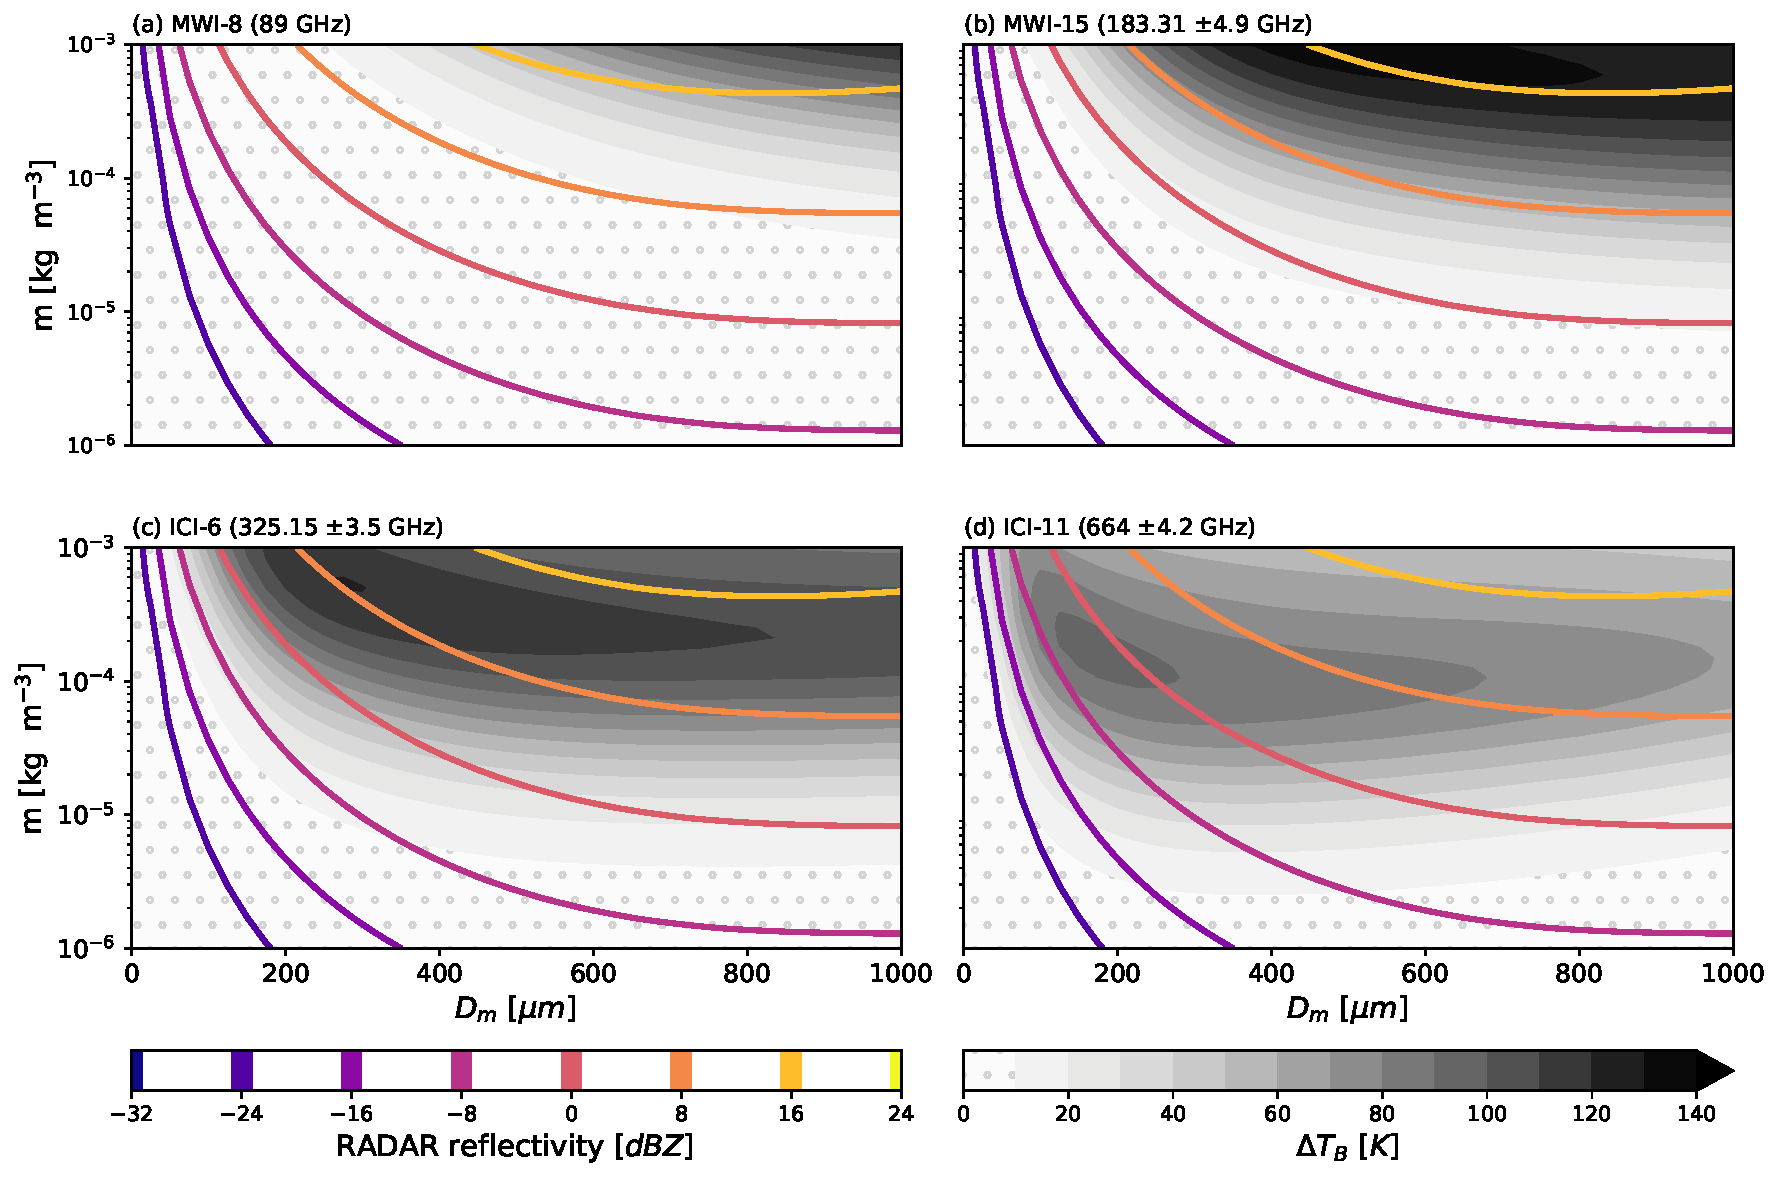
\includegraphics[width = 0.8\textwidth]{../plots/contours}
\caption{Simulated observations of a homogeneous cloud layer with
varying mass density $m$ and mass-weighted mean diameter $D_m$. The panels
display the radar reflectivity in dBZ at the cloud center overlaid onto the
cloud signal measured by selected radiometer channels of the MWI radiometer
(first row) and the ICI radiometer (second row).}
\label{fig:contours}
\end{figure}

The contours of the measured active and passive cloud signals show the ambiguity
of the single-instrument measurements with respect to the parameters of the PSD:
Along these contours the signal does not change, while the cloud composition
does. A necessary condition for the ability of a combined retrieval to resolve
this ambiguity is that the contours of the active and passive signals cross each
other. The panels in Fig.~\ref{fig:contours} thus give an indication to what
extent the information in the radar measurement and the corresponding passive
radiometer channel provide complementary information on the parameters of the
PSD. Considering the panels corresponding to the MWI channels, the results show
that the observations contain complementary information only for very dense
clouds consisting of very large particles. Compared to that, the ICI
observations display a lower degree of parallelism already at lower densities
and particle sizes, indicating higher complementary information content also for
thinner clouds.

\subsection{Retrieval results}

To assess the performance of the combined cloud retrieval, the developed
algorithm has been applied to the two designated cloud scenes. The same
retrievals have been performed with a radar-only and a passive-only version of
the algorithm to serve as baselines for the combined retrieval. Each retrieval
was performed multiple times using different ice particle models. The tested
particle shapes are listed together with the corresponding mass size relations
and ARTS SSDB identifier in Tab.~\ref{tab:particles_retrieval}. Since the
results for both test scenes are qualitatively similar, not all analyses are
shown for both scenes. Instead, these are provided as a digital supplement to
this article.

\begin{table}
  \centering
  \caption{Particle model name, ARTS scattering database ID and parameters
    $\alpha, \beta$ of the mass-size relationships of the particle habits used
    in the retrieval.}
  \begin{tabular}{l|c|c|c}
    Name & ID & $\alpha$ & $\beta$ \\
    \hline
    GemCloudIce         & 31  & 440      & 3 \\
    GemSnow             & 32  & 24.0072  & 2.8571 \\
    GemGraupel          & 33  & 172.7527 & 2.9646 \\
    8-ColumnAggregate   &  8  & 65.4480  & 3      \\
    PlateType1          &  9  & 2.4770   & 0.7570 \\
    LargePlateAggregate &  20 & 2.2571   & 0.2085 \\
  \end{tabular}
  \label{tab:particles_retrieval}
\end{table}

The forward-simulated observations that were generated to test the retrievals
are shown for the first test scene in Fig.~\ref{fig:observations_a}. Independent
Gaussian noise with standard deviations according to sensor specifications has
been added to the simulated observations to account for sensor noise. A source
of forward model error is accounted for in the observations by To model
the forward model error that would affect a real retrieval, the forward
simulations have been performed using the full microphysics from the GEM model.
This means that the synthetic observations were computed using six hydrometeor
classes, while the retrieval forward model uses only two classes of
hydrometeors. Errors due mismatch of sensor footprints or inhomogeneity of the
atmosphere across the fields of view of the sensors are not represented in the
simulated observations.


\begin{figure}
\centering
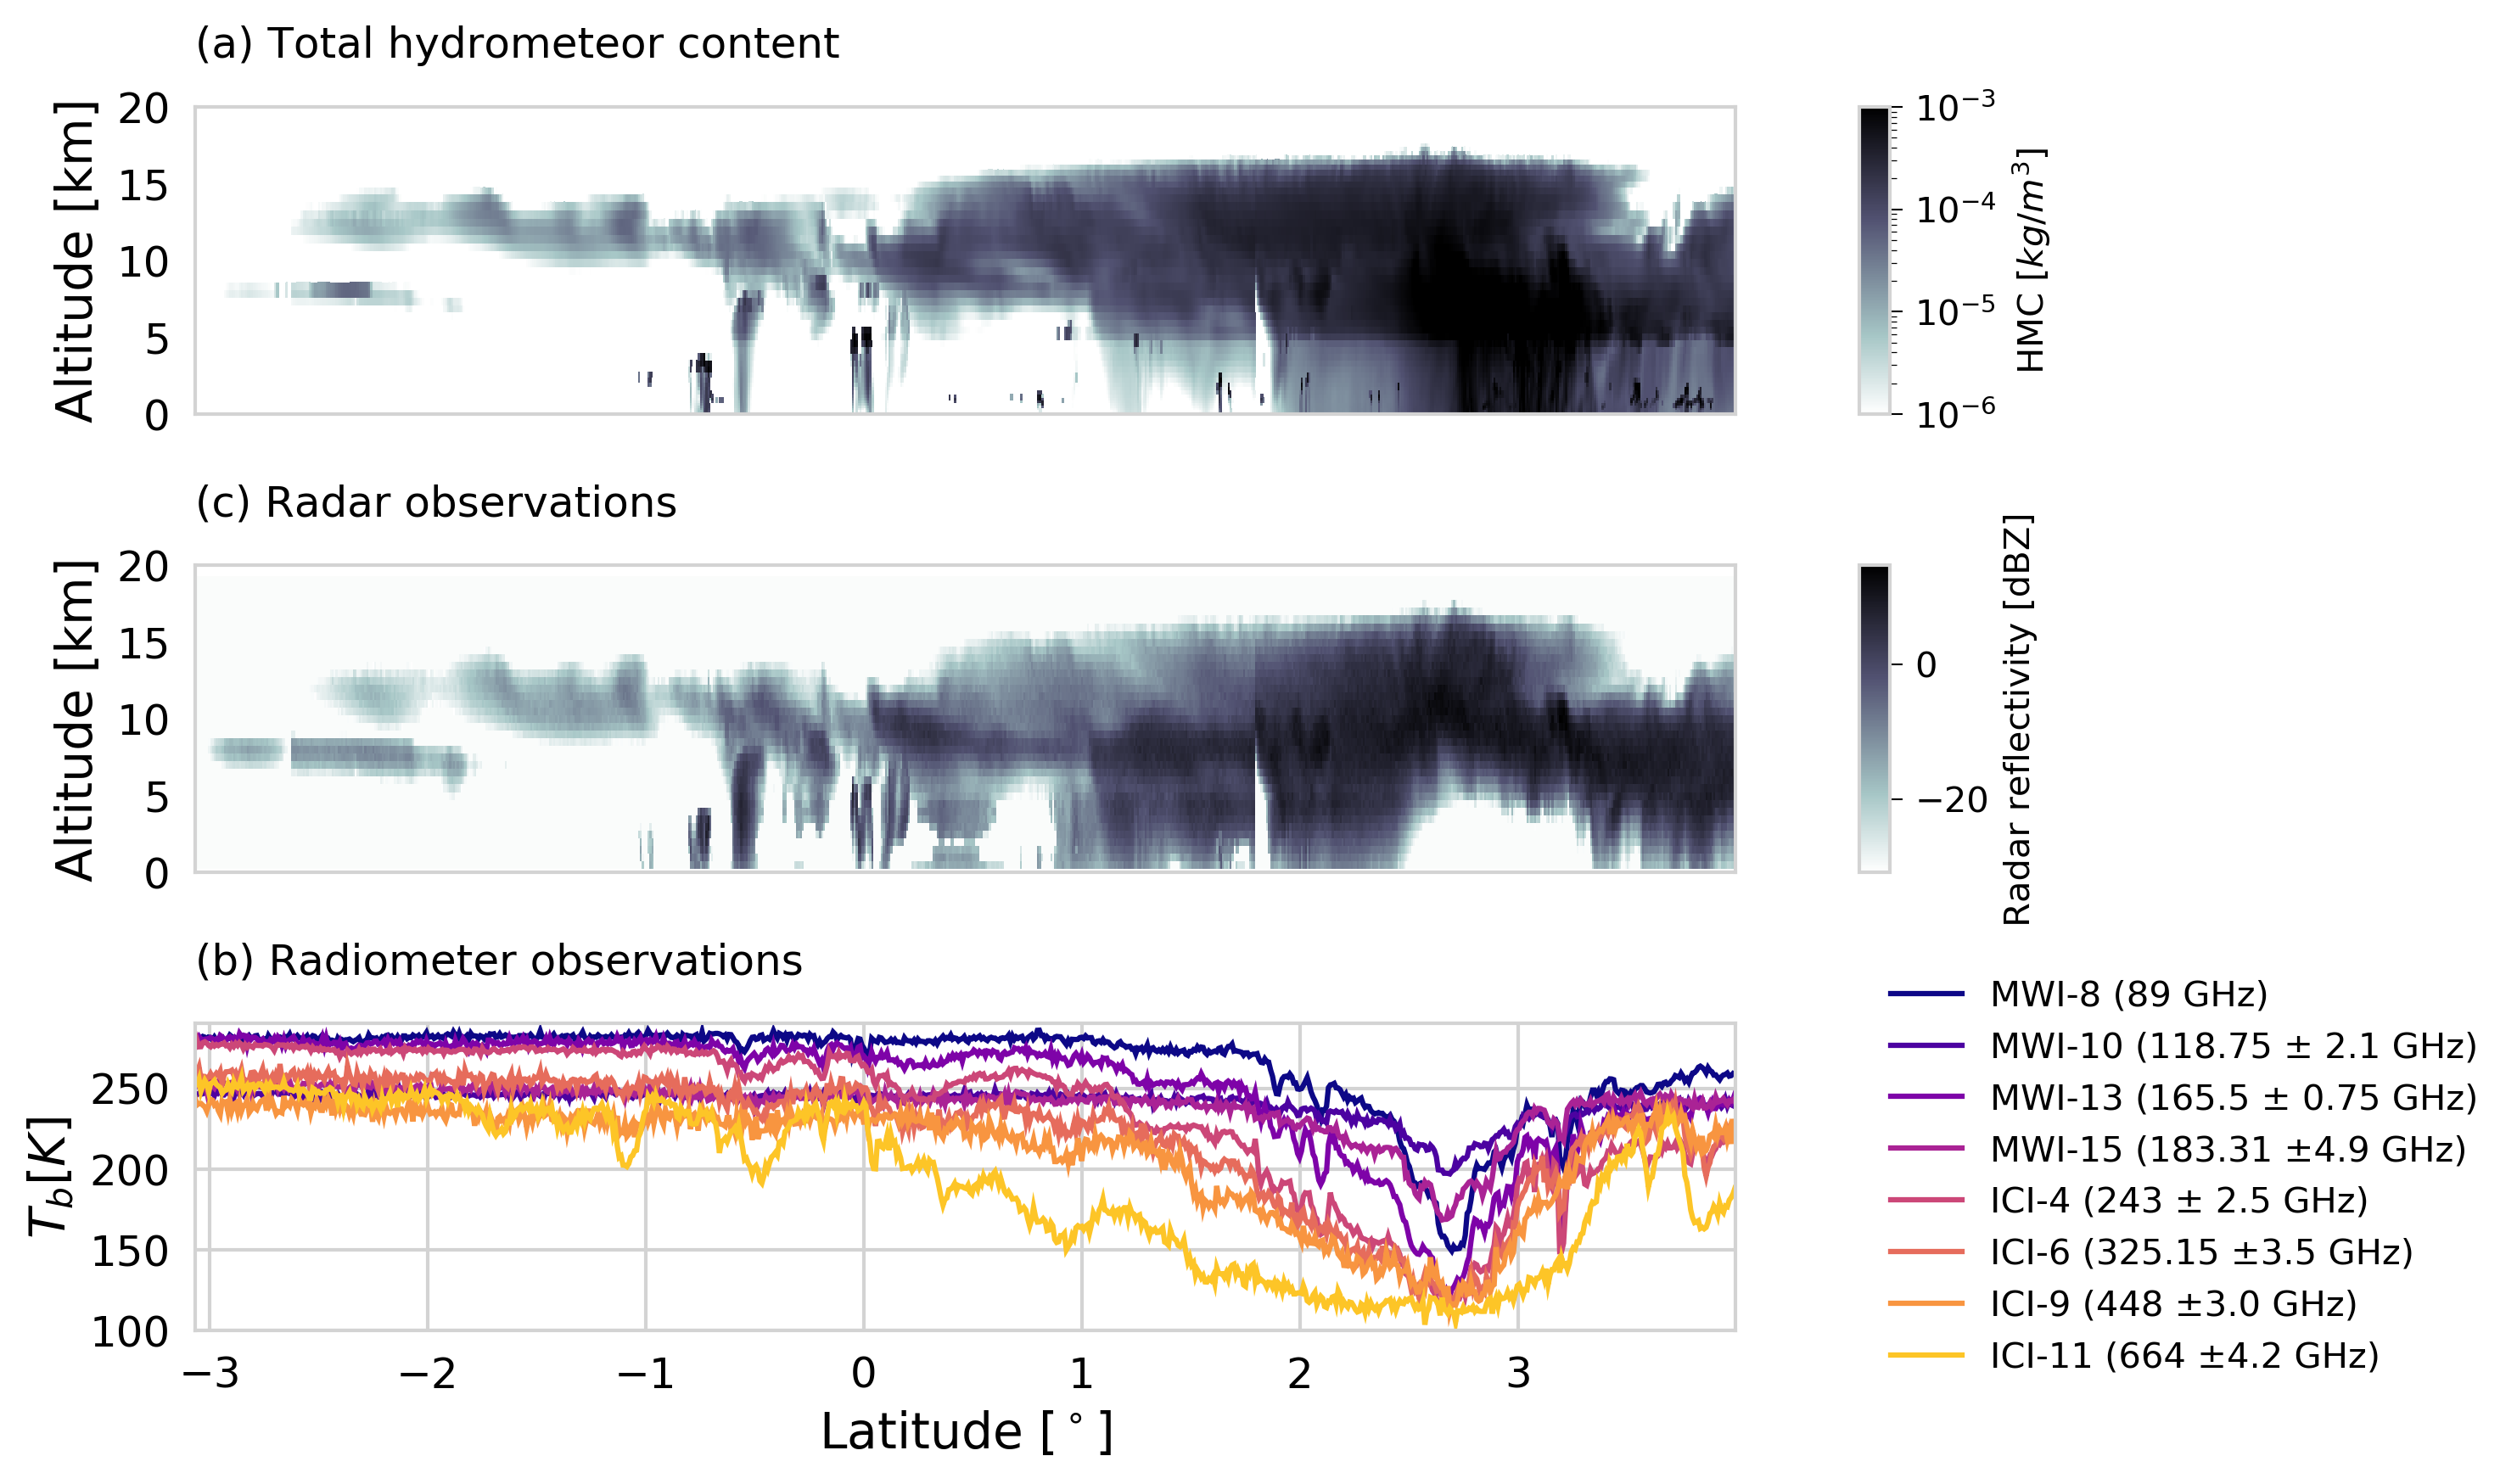
\includegraphics[width = 0.8\textwidth]{../plots/observations_a}
\caption{Total hydrometeor content and simulated observations for the first test
  scene. Panel (a) displays the total hydrometeor content in the scene, i.e. the
  sum of the mass densities of all hydrometeor species of the GEM model. Panel
  (b) shows the simulated radar reflectivities. Panel (c) displays the simulated
  brightness temperatures for a selection of the channels of the MWI and ICI
  radiometers.}
\label{fig:observations_a}
\end{figure}

\subsubsection{Mass concentrations}

To provide an overview over how well the different retrievals are able to
reproduce the cloud structures in the test scene, the retrieved ice water
content (IWC) fields for the first test scene are shown in Figure
\ref{fig:results_a}. The results were obtained using the LargePlateAggregate as
particle model, which was found to give the overall best retrieval performance.

Panel (a) of the figure displays the final value of the OEM cost function $l$
(normalized by the dimension of the measurement space) achieved during the
minimization process. A high final value of $l$ means that no state was found
that agrees well with both the input observations and the a priori assumptions
and thus indicates a low-quality retrieval. A first difference between the three
retrievals becomes apparent from these results: While the radar-only retrieval
achieves a low final cost over almost the whole scene, the passive-only and the
combined retrieval do not achieve a low cost in regions where the cloud is thick
and complex in structure.

Panel (b) displays the retrieved column-integrated IWC, the ice water path
(IWP). The IWP is plotted in $\ \unit{dB}$ relative to the reference IWP in the
scene since the curves could otherwise not be distinguished due to the high
dynamic range of the reference values. Although quite noisy, the combined
retrieval yields the lowest deviations in the retrieved IWP over large parts of
the scene except for the regions where the retrieval failed to find a good fit
to the observations.

Panel (c) shows the IWC field retrieved using the passive-only retrieval.
Although there are similarities to the reference mass concentration, the results
do not reproduce the vertical structure of the cloud very well. It should be
noted, however, that the displayed mass-density range extends below the
sensitivity limit of the passive-only observations around
$10^{-5}\ \unit{kg/m^3}$ (c.f. Fig. ~\ref{fig:contours}), which explains the
smeared-out appearance of the results to some extent.

In contrast to this, the radar-only results, shown in panel (d), reproduce the
vertical structure of the cloud well. Nonetheless, when compared to the
reference mass concentration field, certain discrepancies are visible: The
radar-only retrieval tends to overestimate the mass density at the bottom
of the cloud and underestimate the mass concentrations at the top of the cloud.

The results of the combined retrieval are displayed in panel (e). Although some
artefacts are clearly visible in the retrieved mass density field, the retrieval
still reproduces the vertical structure well. In particular, the combined
retrieval succeeds to correct some of the systematic deviations of the
radar-only retrieval: The mass at cloud base is reduced and increased at cloud
top.


\begin{figure}
\centering
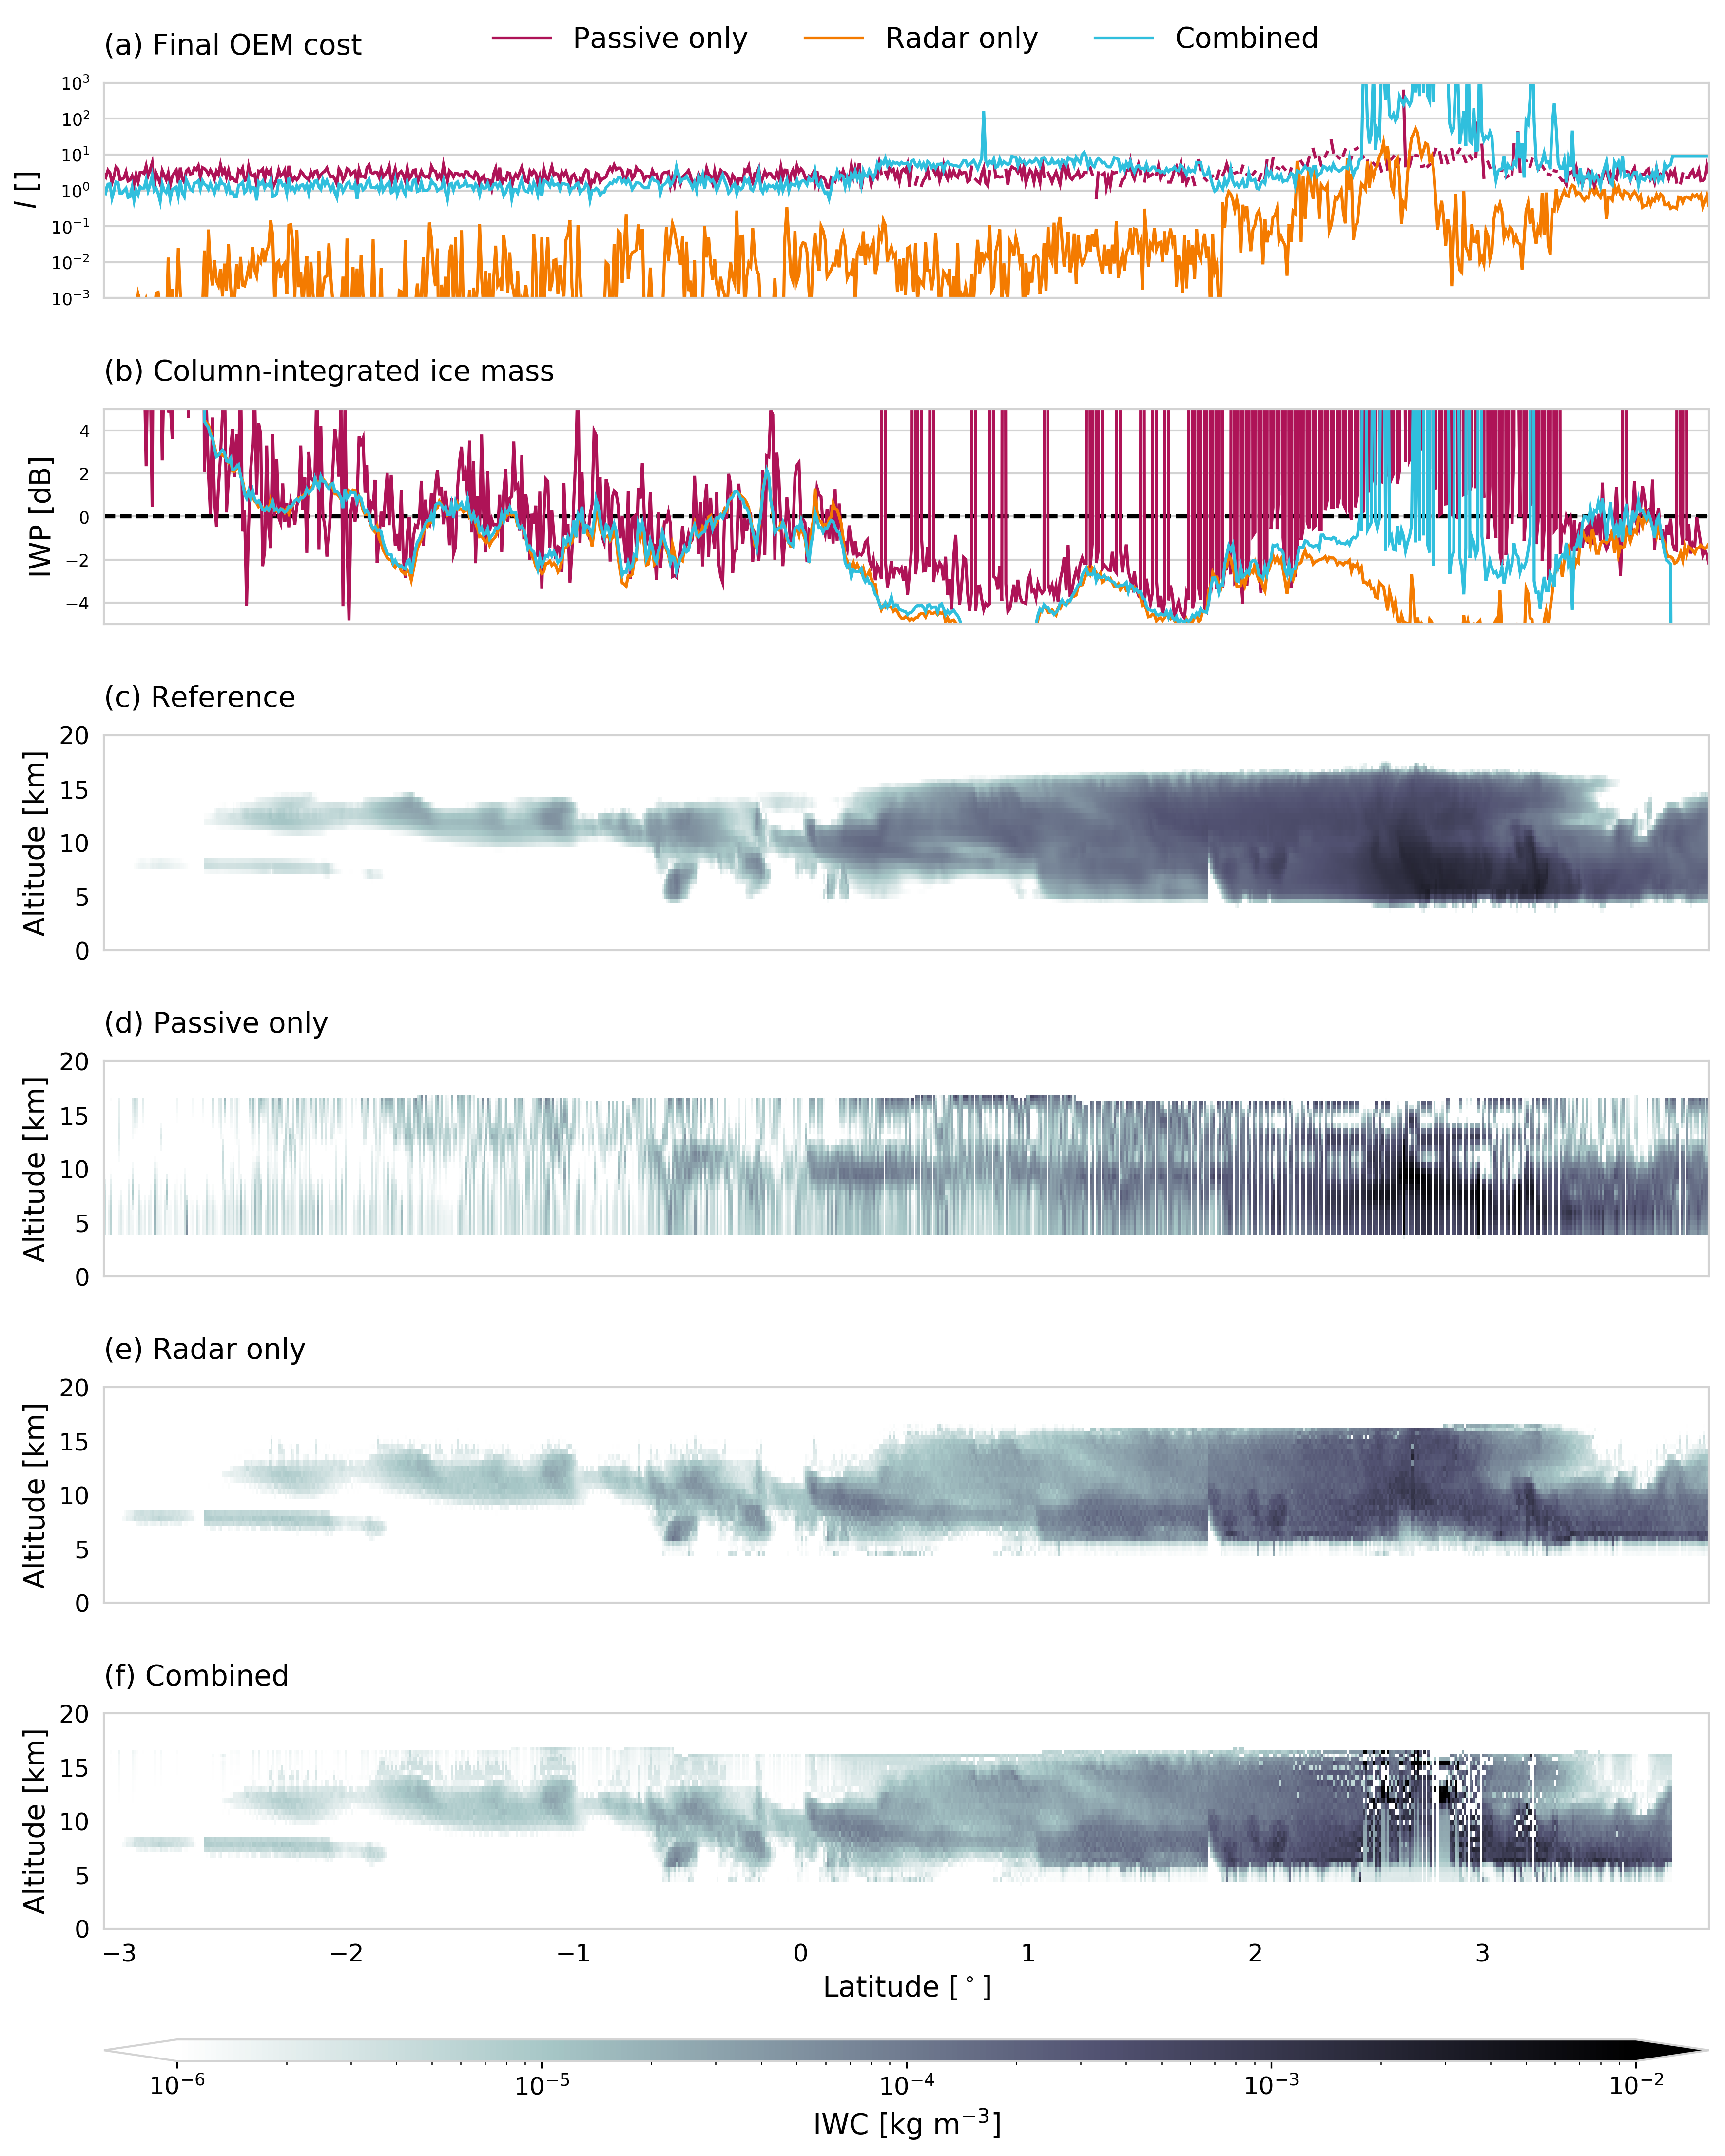
\includegraphics[width = 0.8\textwidth]{../plots/results_a_LargePlateAggregate}
\caption{Reference and retrieved mass concentrations of frozen hydrometeors for
 the first test scene. Panel (a) displays the final OEM costs achieved during
 the minimization normalized by the number of dimensions of the measurement
 space. Panel (b) displays the reference mass concentrations from the model
 scene. Panel (c), (d) and (e) display the retrieval results for the
 passive-only, radar-only and combined retrieval.}
\label{fig:results_a}
\end{figure}

To make the assessment of the retrieval performance more quantitiave, the
reference mass concentrations are plotted against the retrieved values in
Fig.~\ref{fig:results_scatter_a_1} and \ref{fig:results_scatter_a_2}. The plots
show the results for all different retrieval configurations and tested
particle models. Markers in the plots are color-coded according to the
prevailing hydrometeor type (by mass density) in the reference scene, in order
to allow assessment of the retrieval performance for the different hydrometeor
types of the GEM model.

Not surprisingly, the results from the passive-only retrieval exhibit the
strongest deviations from the diagonal. Since the passive channels alone contain
only limited information on the vertical distribution of ice in the atmosphere,
the retrieval cannot be expected to yield accurate results at the resolution
considered here. Although rather weak, a certain effect of the ice particle
model on the retrieval results can be observed. In particular, the GemCloudIce
leads to a systematic underestimation of ice mass densities, that are less
pronounced for the other particle models.

\begin{figure}
\centering
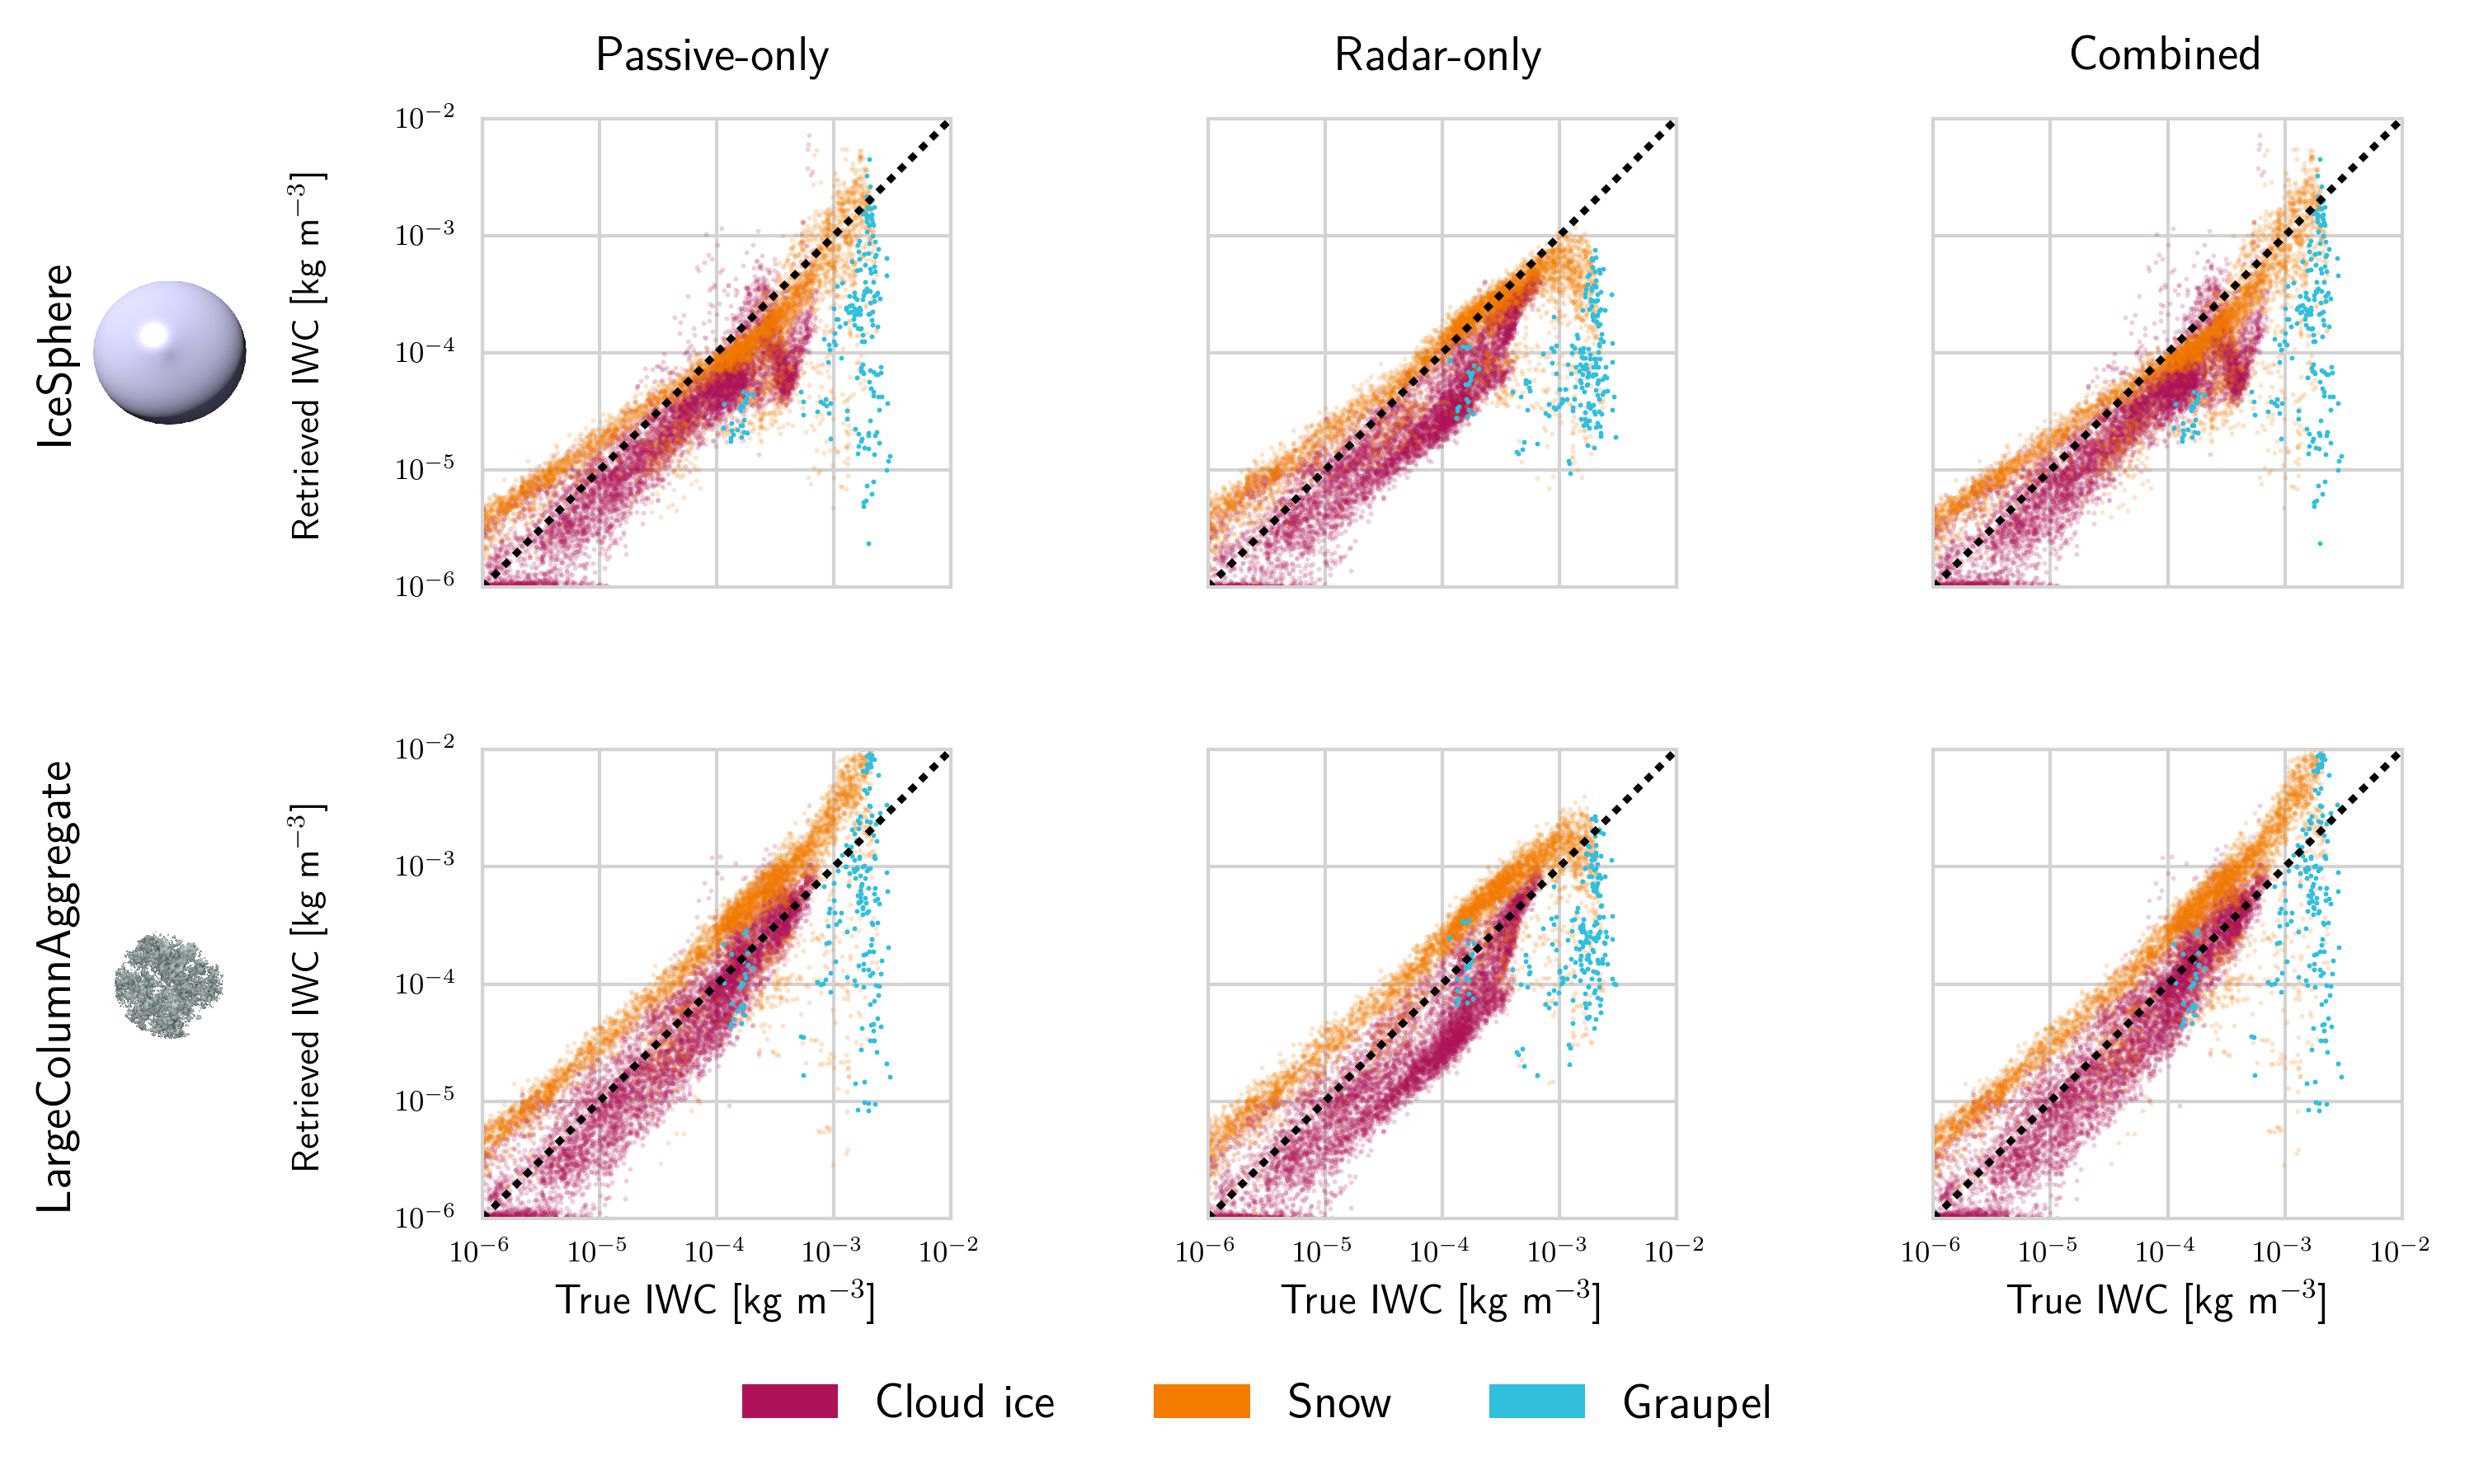
\includegraphics[width = 0.8\textwidth]{../plots/results_scatter_a_1}
\caption{Reference mass concentrations plotted against retrieved mass
  concentrations for the tested retrieval configurations. Each row shows the
  retrieval results for the particle shape shown in the first panel of each row.
  The following panels show the retrieval results for the passive only (second
  column), the radar only (third column) and the combined retrieval (fourth
  column). Markers are colored according to the prevailing hydrometeor type at
  the corresponding grid point in the reference scene. Due to their sparsity,
  marker corresponding to hail are drawn at twice the size of the other
  markers.}
\label{fig:results_scatter_a_1}
\end{figure}

The results from the radar-only retrieval are more accurate than the
passive-only retrieval, with almost all retrieval results located fairly close
to the diagonal. The most distinct feature of the radar-only results, however,
is the emergence of two clusters that extend along the diagonal but are
displaced above respectively below it. The color coding of the markers reveals
that these clusters correspond to grid points dominated by ice for the clusters
below the diagonal and snow for the cluster located above the diagonal. This
indicates that the radar-only retrieval systematically underestimates mass
densities for cloud ice but overestimates the mass density of snow. The effect
is observed for all tested particle shapes indicating that isn't related to
the assumed ice particle shape. In general, the radar-only results exhibit only
very weak dependency on the particle model, making the radar-only results for
different particle shapes virtually indistinguishable.

Another feature that stands out in the radar-only results, is that the retrieval
does not work for graupel. This, however, can be understood by comparing the
radar reflectivities shown in Fig.~\ref{fig:observations_a} with the cloud
structure displayed in Fig.~\ref{fig:overview}. It becomes apparent that graupel
in this scene is located where the radar signal is fully attenuated. Since there
is no signal to retrieve the mass density from, this explains the bad
performance of the radar-only retrieval for these grid points.

Similar as the radar-only retrieval, the results of the combined retrieval are
located close to the diagonal. However, the clusters observed in the radar-only
result are to large extent merged in the combined results. Moreover, except for
the results obtained with the GemCloudIce particle shape, the two clusters move
in closer towards the diagonal. This improved retrieval performance of the
combined retrieval, clearly indicates that the complementary information content in
the passive observations helps to better constrain the cloud microphysics in the
different regions of the cloud.

Nonetheless, the results for the GemCloudIce particle stand out in the results.
Even though the systematic deviations observed in the radar-only retrieval are
reduced for most particle shapes, for this specific shape they are instead
increased. The retrieval error is particularly large for snow, which is strongly
underestimated for reference mass concentrations around $10^{-4} \ \unit{kg/m^3}$.

\begin{figure}
\centering
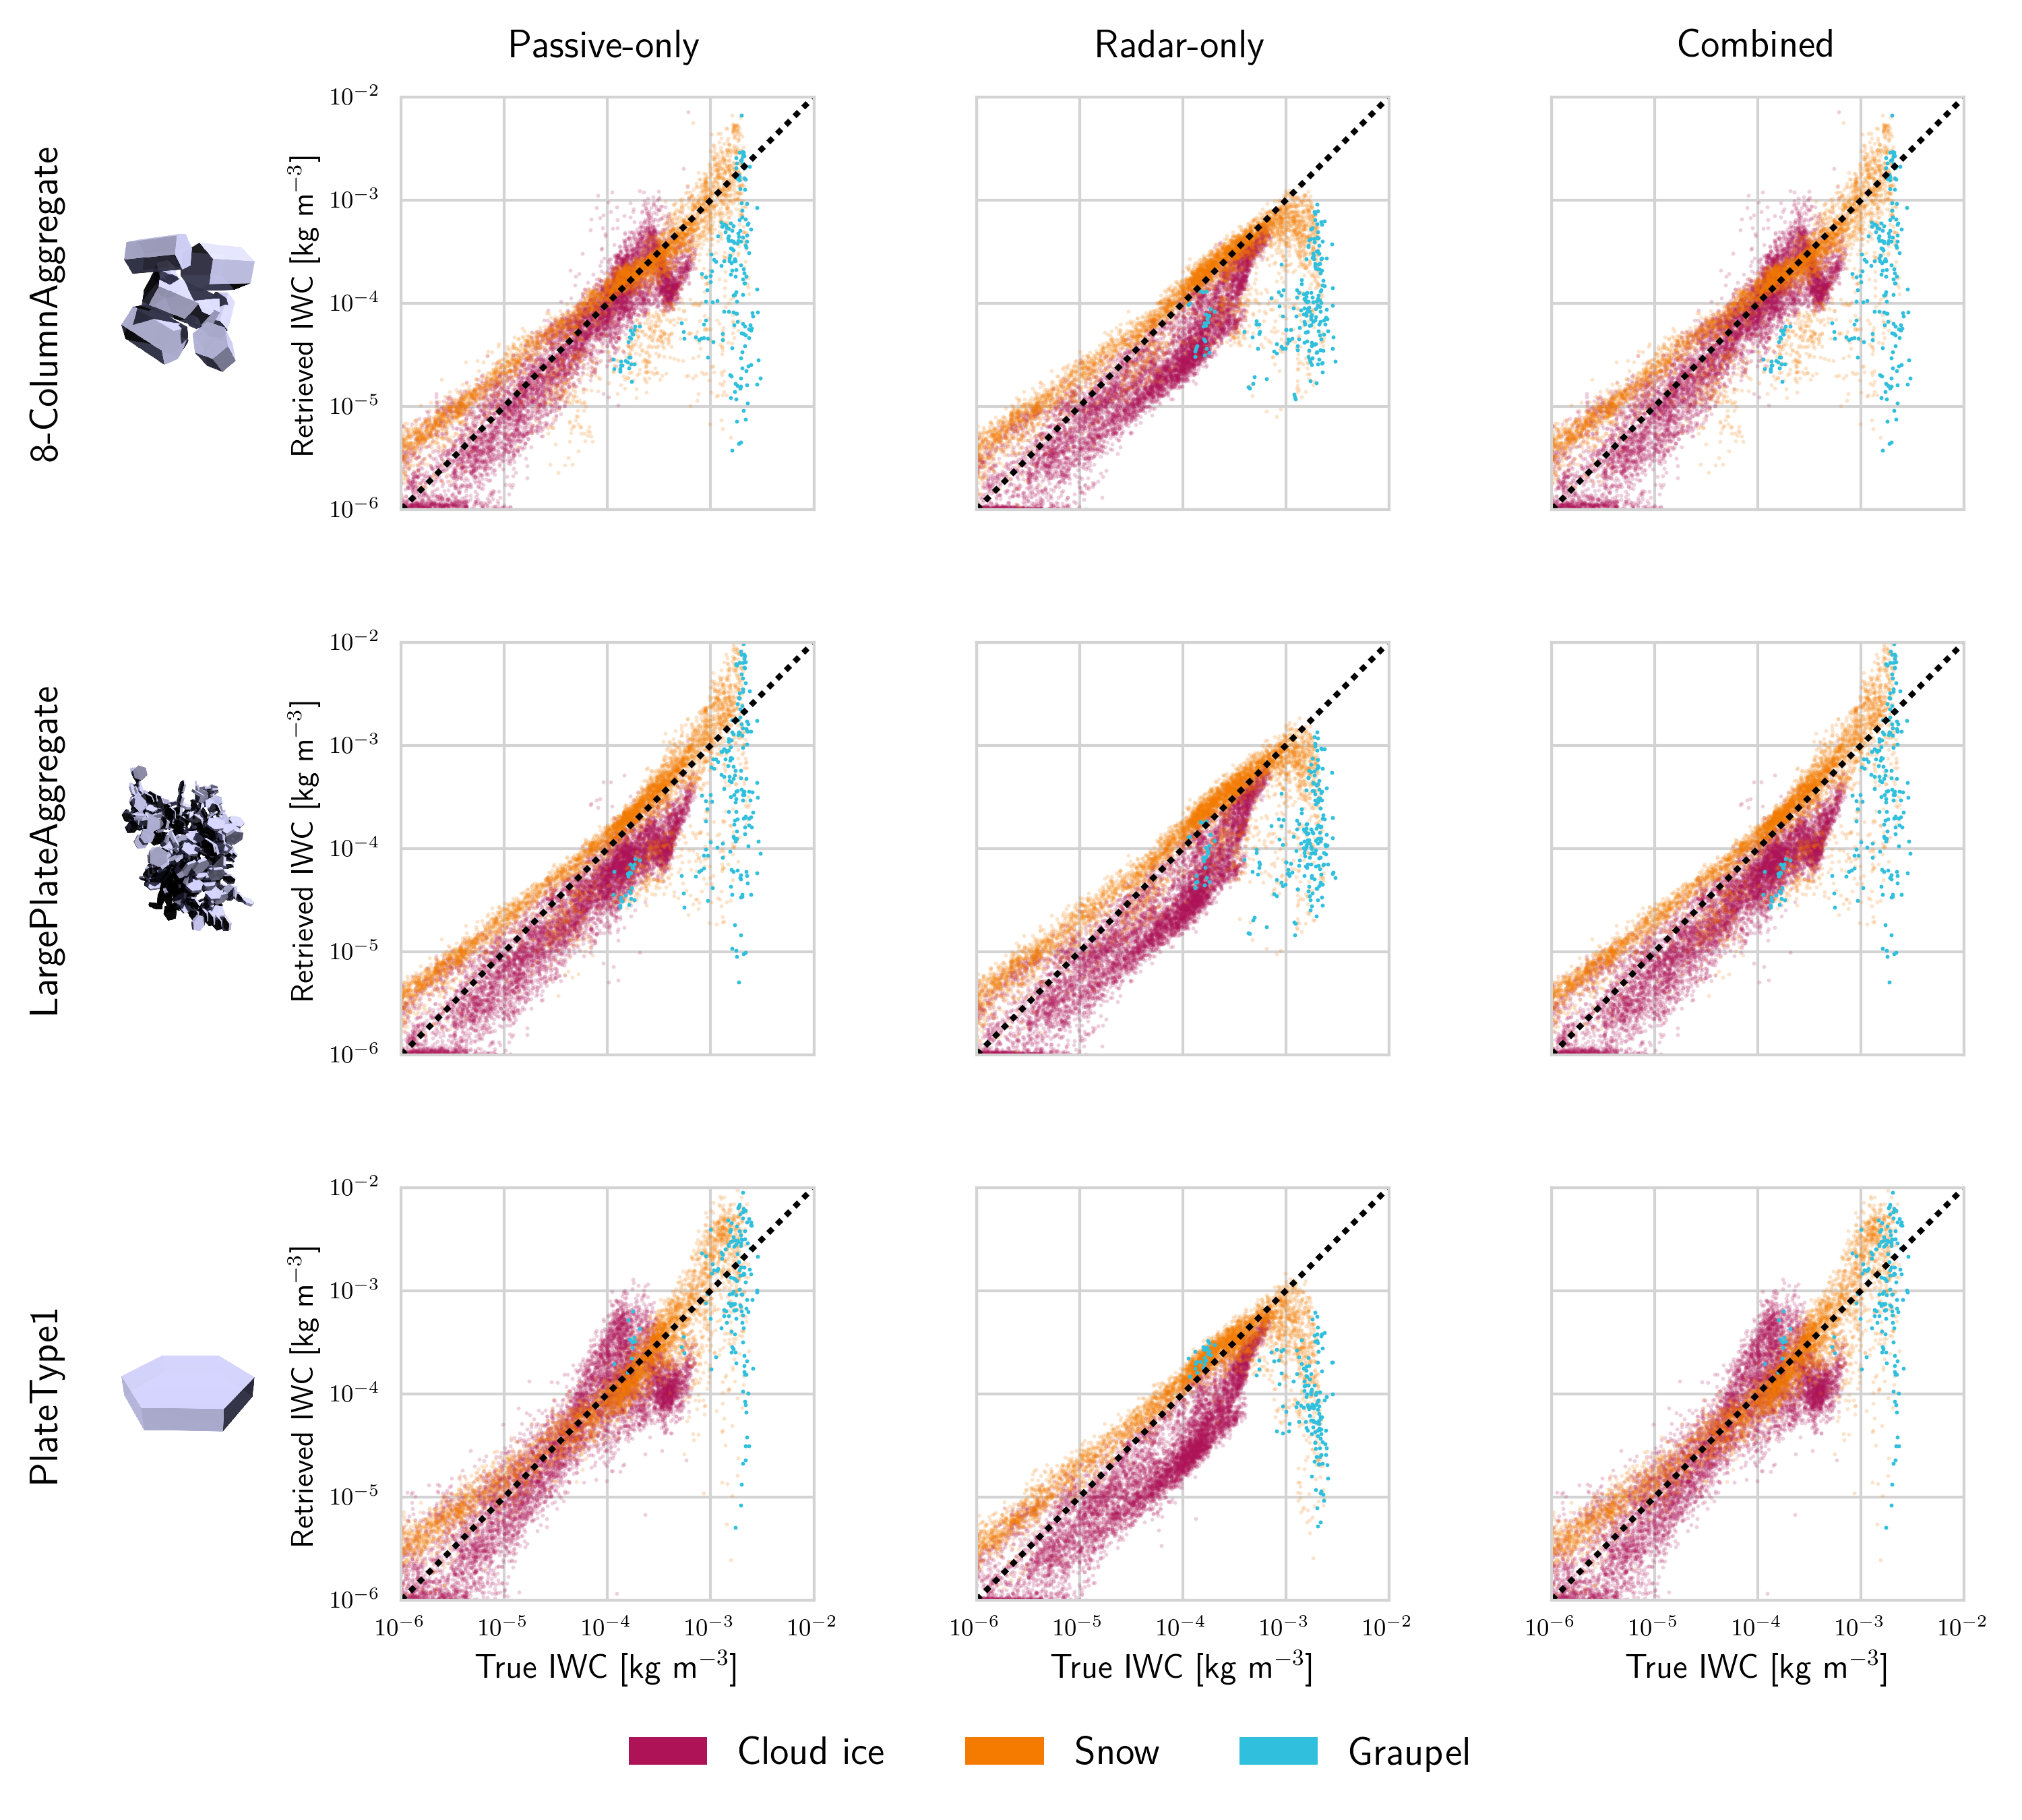
\includegraphics[width = 0.8\textwidth]{../plots/results_scatter_a_2}
\caption{Same as Fig.~\ref{fig:results_scatter_a_1} but for the remaining particle
  shapes.}
\label{fig:results_scatter_a_2}
\end{figure}


The results for the second test scene obtained using the LargePlateAggregate
particle model are shown in Fig.~\ref{fig:results_b}. As mentioned above, the
results are qualitatively very similar to those of the first scene. Also here,
the final OEM cost, shown in Panel~(a), displays a region of increased cost for
the passive-only and combined retrievals. This is again a region of very dense
cloud that consists of graupel and snow. Also similar to the first scene, the
passive only retrieval does not reproduce the structure of the cloud well.
Although the cloud top is placed at the right position neither the vertical
structure of the cloud nor its base are resolved. The radar-only retrieval
resolves the vertical structure of the cloud well, but overestimates the ice
mass density in the scene. The combined retrieval also resolves the vertical
structure of the cloud well and corrects the overestimation observed in the
radar-only results to some extent.

\begin{figure}
\centering
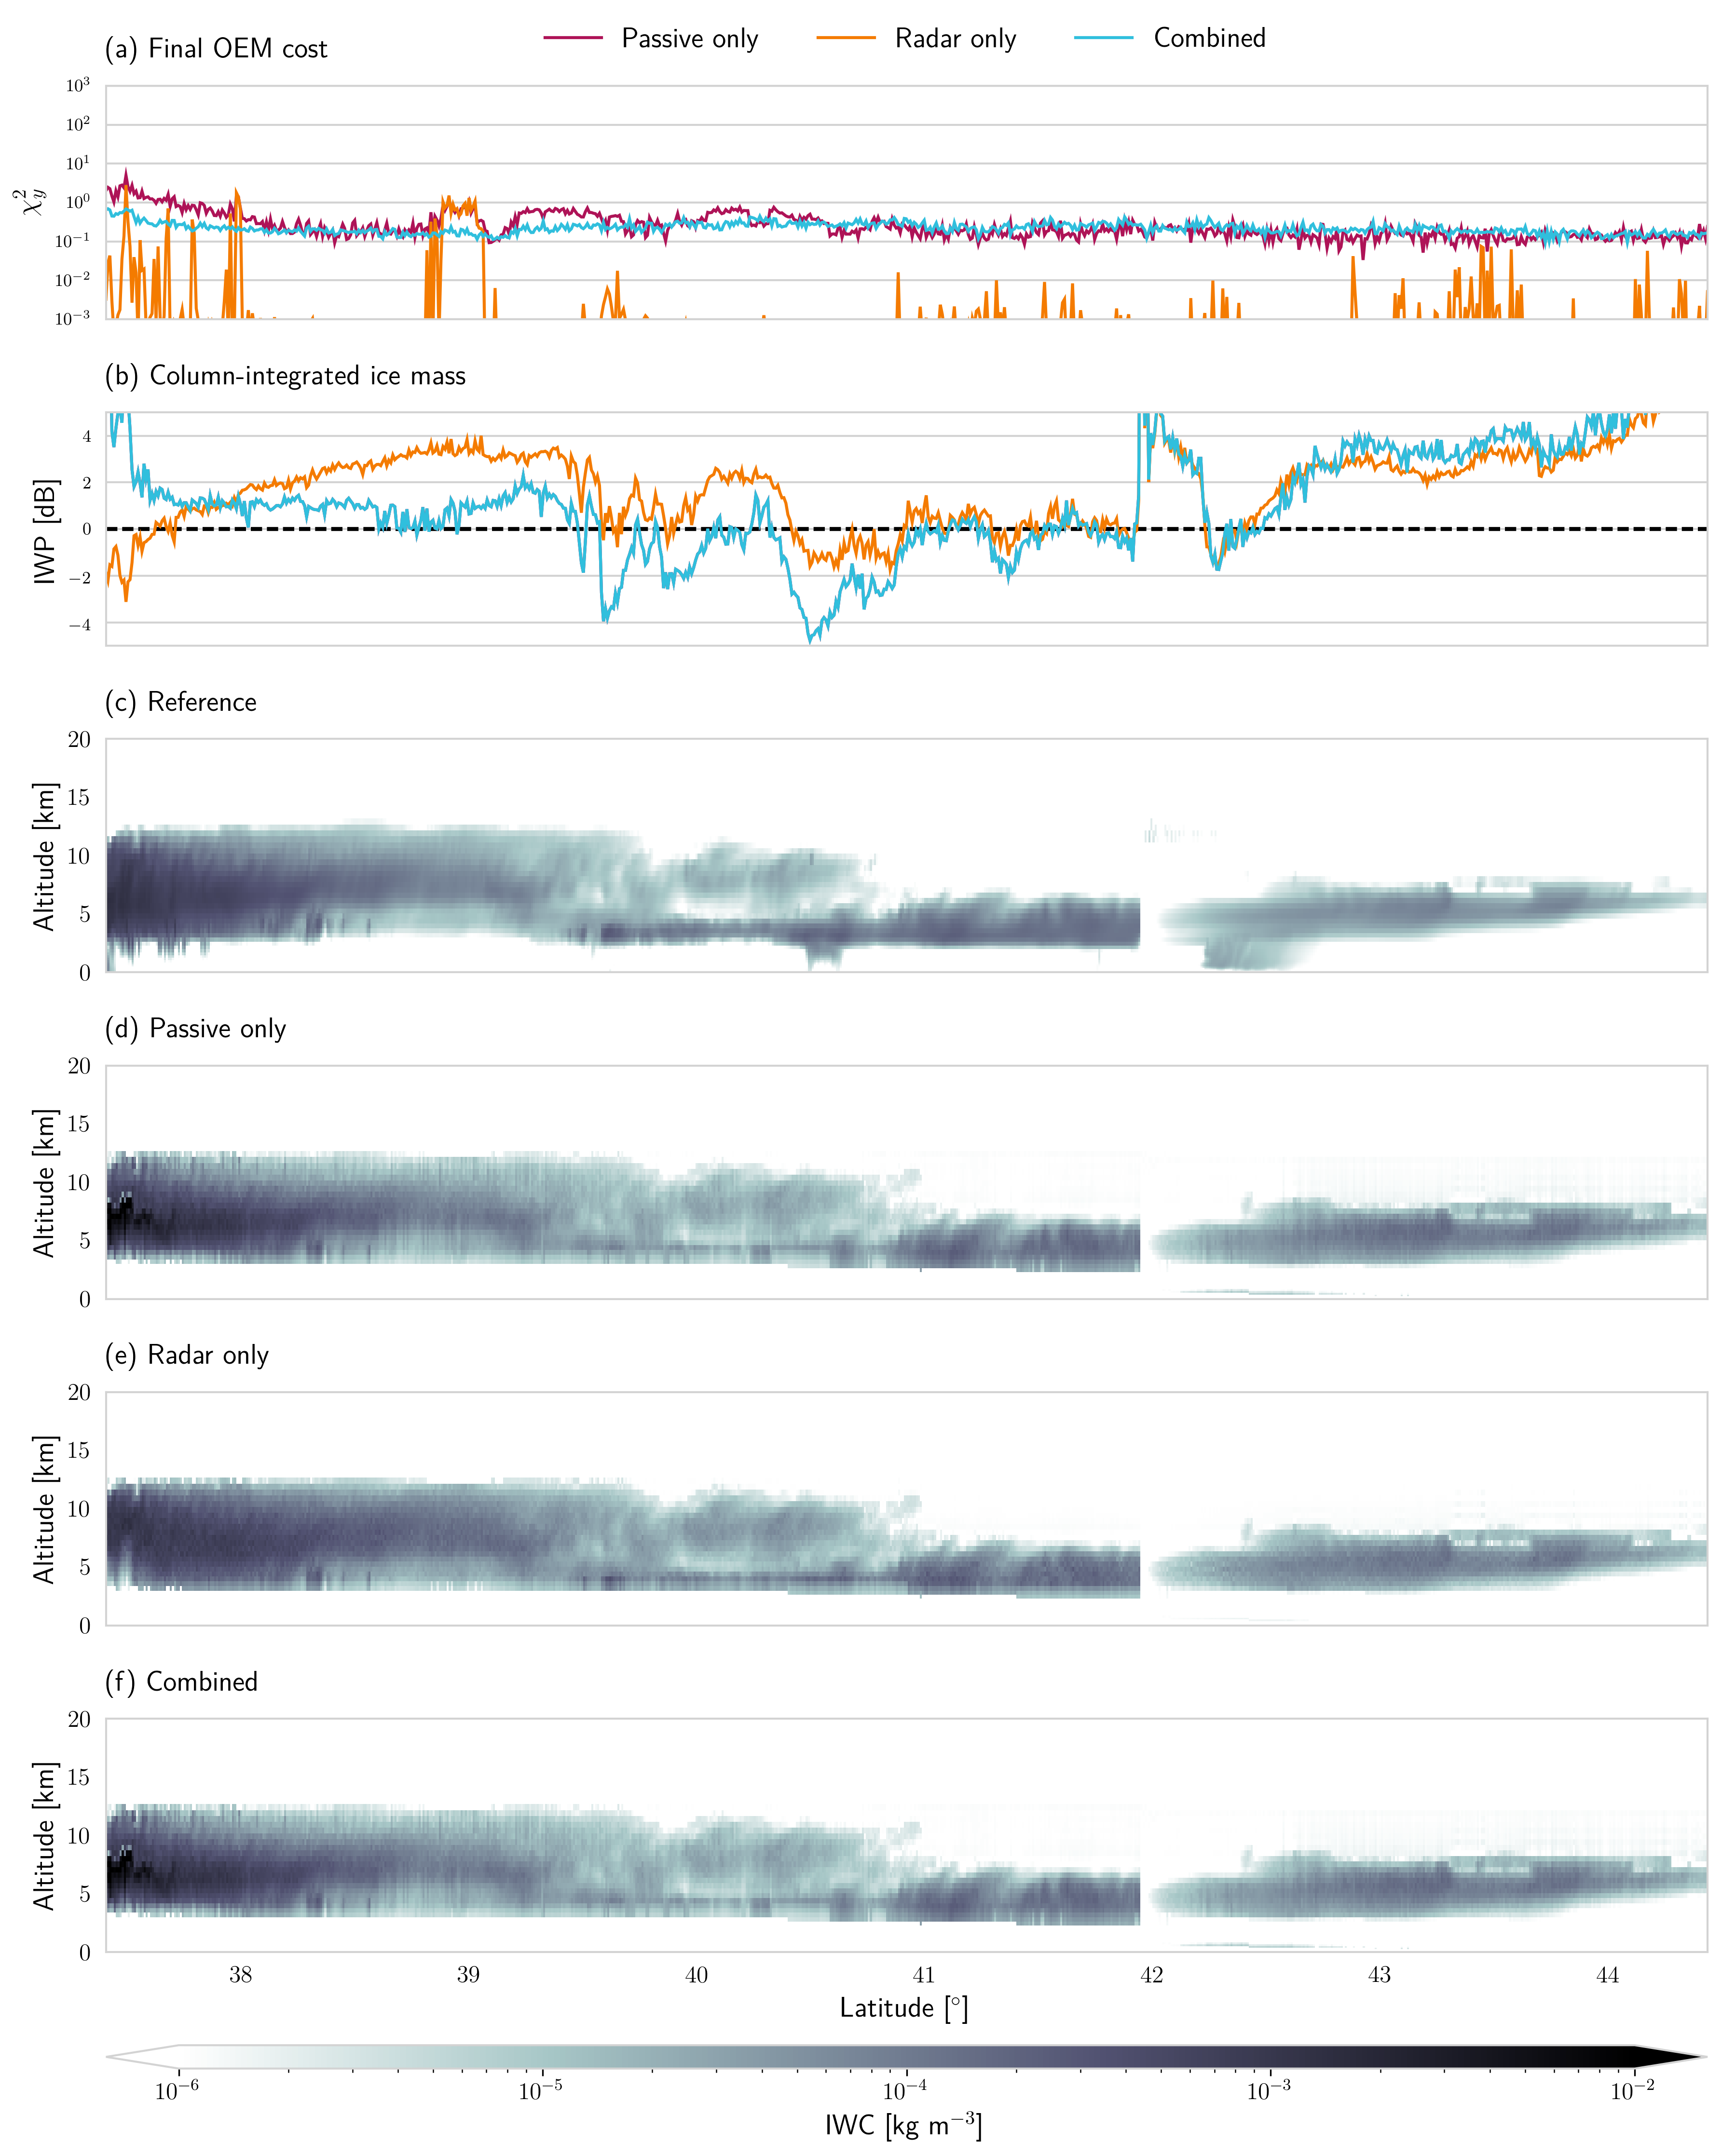
\includegraphics[width = 0.8\textwidth]{../plots/results_b_LargePlateAggregate}
\caption{Reference and retrieved mass concentrations of frozen hydrometeors for
 the second test scene. Panel (a) displays the final OEM costs achieved during
 the minimization normalized by dimensions of the measurement space. Panel (b)
 displays the reference mass concentrations from the model scene. Panel (c),
 (d) and (e) display the retrieval results for the passive-only, radar-only
 and combined retrieval.}
\label{fig:results_b}
\end{figure}

Scatter plots for the retrieval results from the second scene are shown in
Fig.~\ref{fig:results_scatter_b_1}. Except for the lack of cloud ice in the
scene, the results are the same as what has been observed in the first scene:
The radar-only retrieval overestimates the mass density of snow in the scene.
This effect is corrected by the combined retrieval for most of the tested
particle shapes. The exception is the GemCloudIce particle for which the
retrieval of snow particle deteriorates quite drastically.

\begin{figure}
\centering
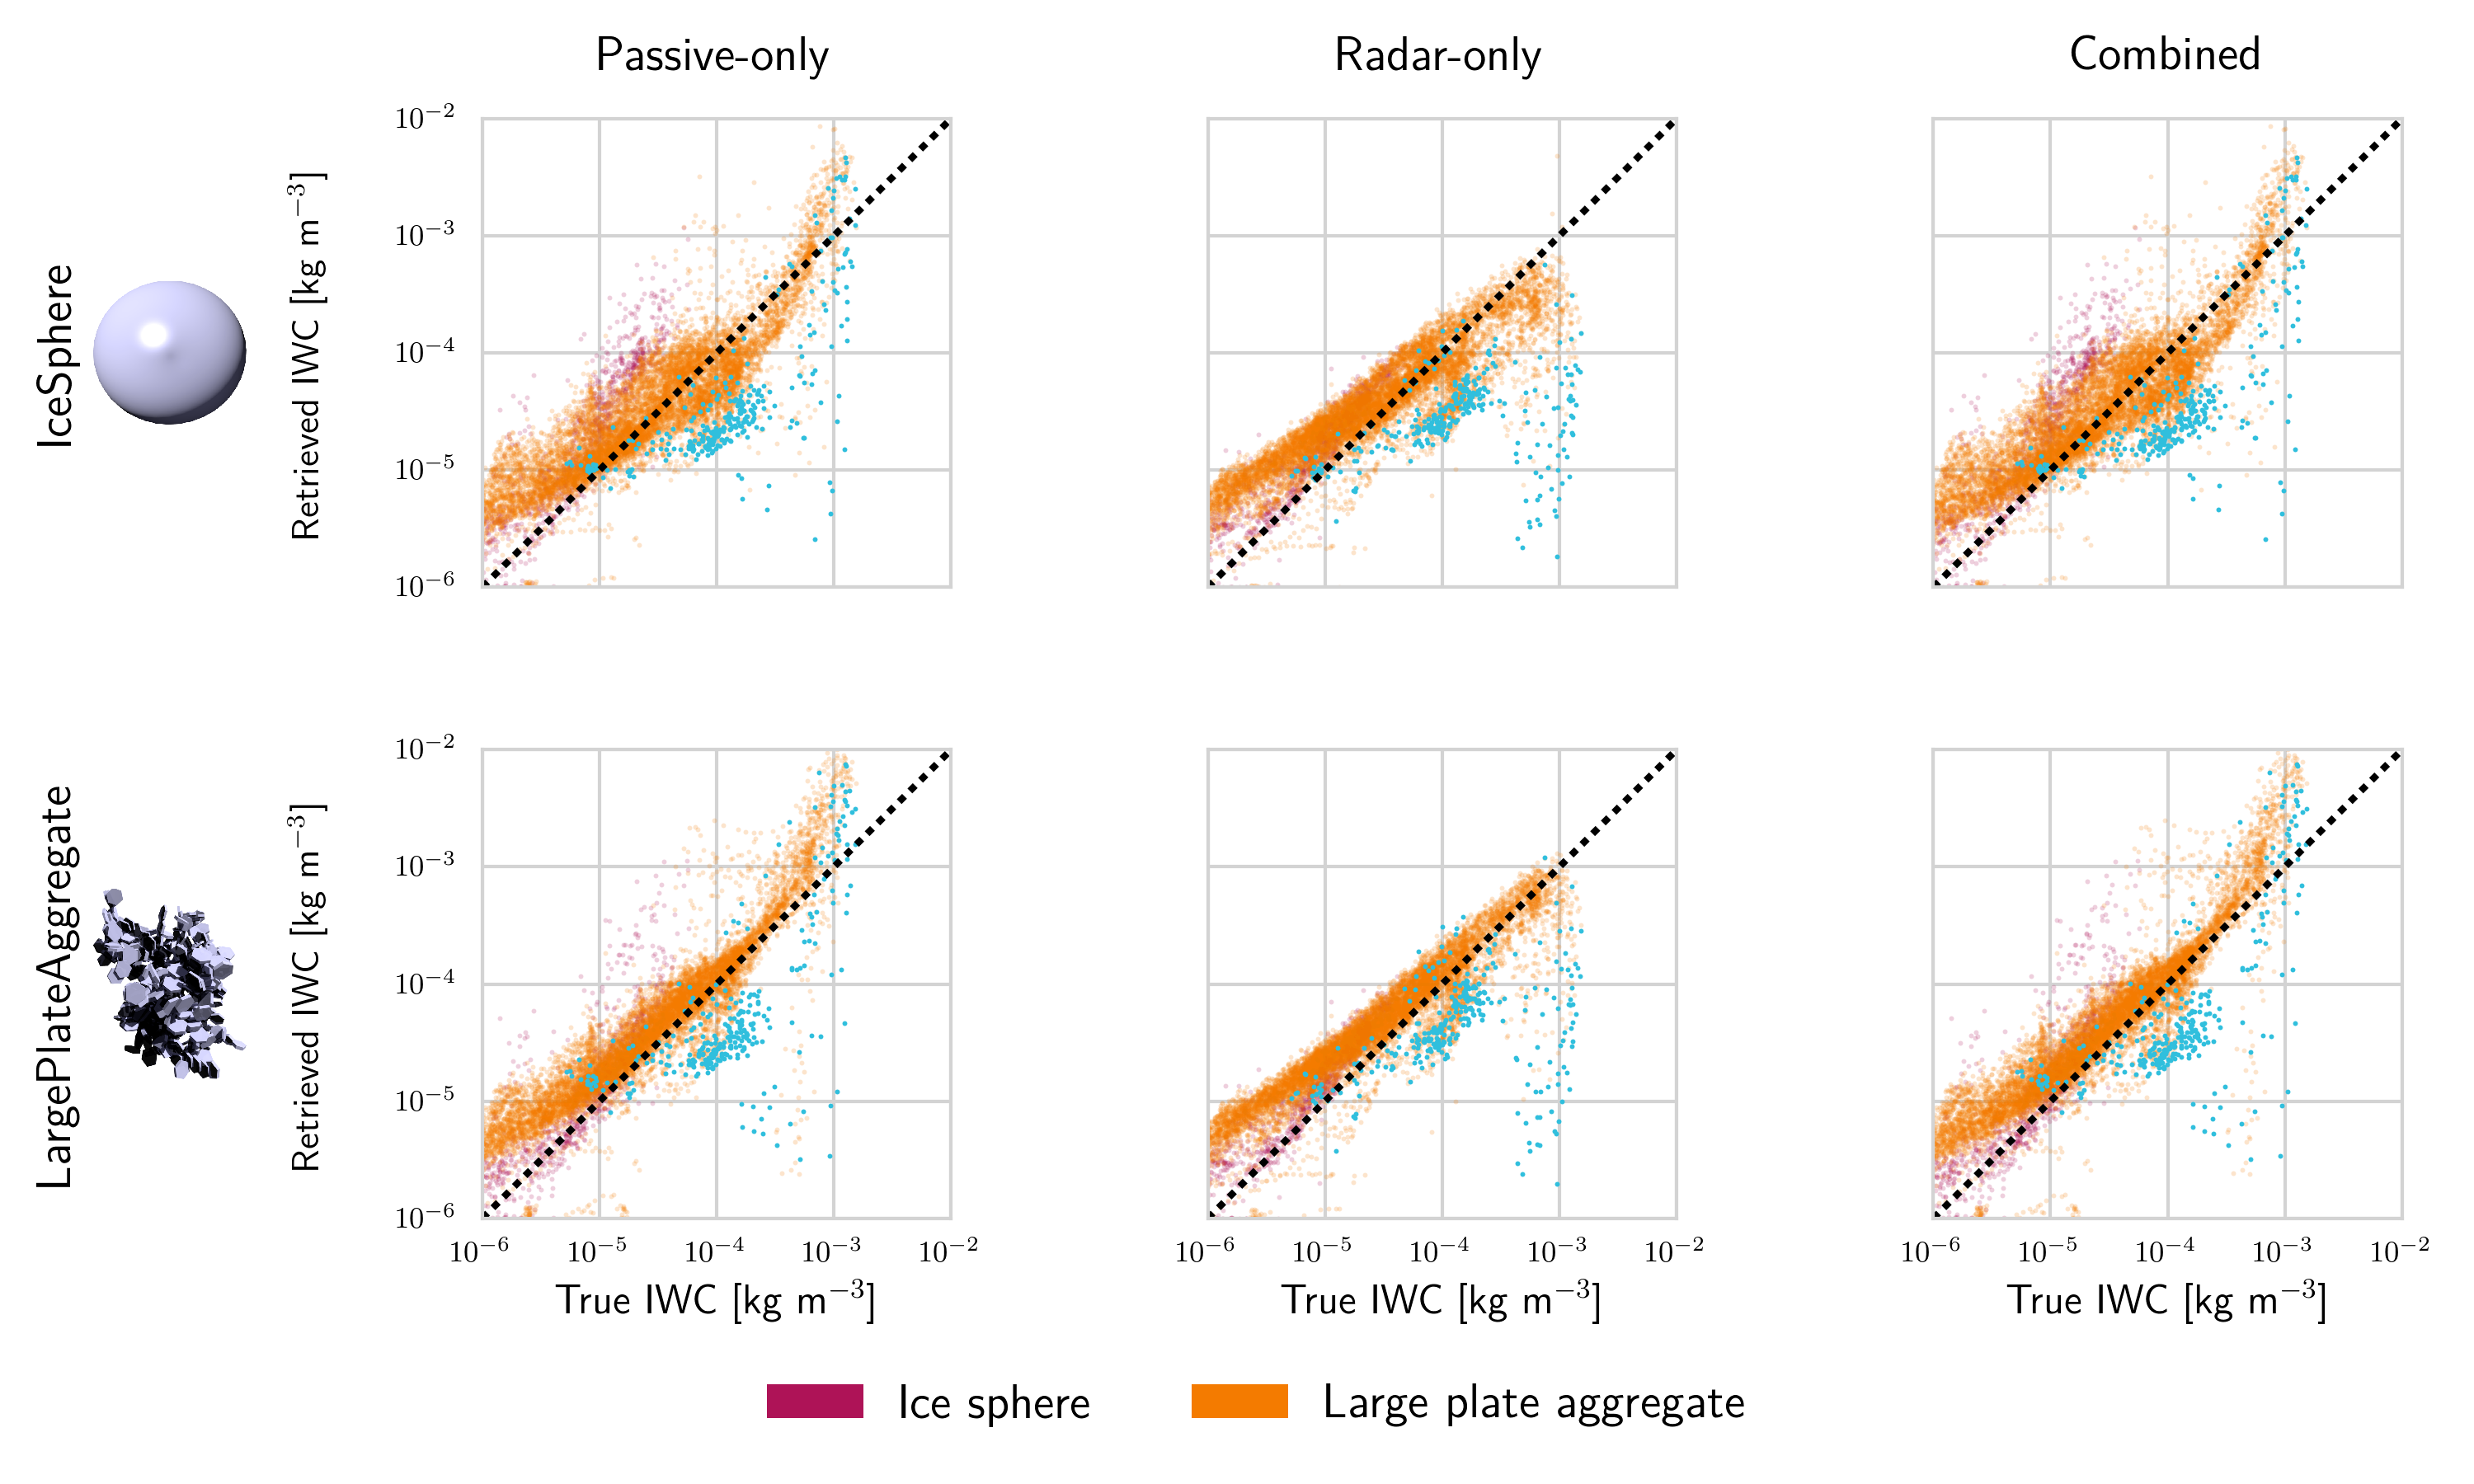
\includegraphics[width = 0.8\textwidth]{../plots/results_scatter_b_1}
\caption{Scatter plots of the reference and retrieved ice mass densities for
  the second test scene. The rows show the retrieval results for a given
  assumed ice particle model. The first column of each row displays a rendering
  of the particle model. The following rows display the results for the
  passive-only, the radar-only and the combined retrieval.}
\label{fig:results_scatter_b_1}
\end{figure}


\subsubsection{Particle number densities}

A further interesting question is whether and to what extent the joint
observations can improve the retrieval of particle number concentrations.
To address it, particle number densities have been computed from the
retrieved parameters by computing the zeroth moment of the PSD. The resulting
particle number density fields are displayed together with the reference
field in Fig.~\ref{fig:results_nd_a}.

Comparing the passive-only and the radar-only retrieval to the reference
field, the results show that both methods lack skill in predicting number
density concentrations. The strong gradient between the very high concentrations
at the top of the cloud and the low concentrations at the bottom is not resolved
by either of the methods. The combined retrieval, however, manages to reproduce
this gradient in most parts of the scene. Although its exact structure
is not fully reproduced, this clearly shows sensitivity of the retrievals to
the number density concentrations.

Of interest is also the part of the scene where the combined retrieval shows the
strongest deviations from the reference field, that is between $2$ and
$3\ \unit{^\circ}$ latitude. Here, the results strongly underestimate the true
number concentrations. Comparison with the cloud composition displayed in Panel (a)
of Fig.~\ref{fig:overview} shows that this region contains large amounts of both
cloud ice and snow. Since the retrieval uses only a single hydrometeor species
to represent ice in the atmosphere, it is not able to represent such
heterogeneous conditions. Since snow will have the stronger impact on the
observations, the retrieval in these regions tends to predict snow rather than
ice, which leads to the low retrieved number densities.

\begin{figure}
\centering
\includegraphics[width = 0.7\textwidth]{../plots/results_nd_a_LargePlateAggregate}
\caption{Reference and retrieved particle number concentrations of frozen
  hydrometeors for the first test scene obtained with the LargePlateAggregate
  particle model. Panel (a) displays the reference mass concentrations from the
  model scene. Panel (b), (c) and (d) display the retrieval results for the
  passive-only, radar-only and combined retrieval.}
\label{fig:results_nd_a}
\end{figure}

Figure~\ref{fig:results_nd_scatter_a} displays scatter plots of the reference
and retrieved number density concentrations for all three methods and two
particle models from the first test scene. Markers in the plot are color coded
according to their homogeneity, here defined as the ratio of the maximum mass
density of any of the frozen hydrometeor species in the model and the total mass
density. The color coding reveals the emergence of two clusters in the results:
One located at low reference particle number concentrations corresponding to
snow and one at high number concentrations corresponding to regions where the
cloud consists of cloud ice or graupel.

The results confirm that the radar-only retrieval does not exhibit any skill in
retrieving particle number densities. The passive-only results, however, seem to
indicate at least some sensitivity since the cluster corresponding to snow is
placed correctly on the diagonal. In contrast to that, the combined retrieval
moves both clusters towards the diagonal, indicating that it is capable of
distinguishing the microphysical differences of cloud ice and snow. Yet still,
the accuracy of the combined retrieval remains very low.

The effect of particle shape on the retrieval results is similar to what has
been observed for the mass density retrievals. The GemCloudIce model yields the
worst retrieval results, leading to a general underestimation of the true
particle number density. Results for the other particles are mostly similar,
which is why only the result for the LargePlateAggregate is shown here.

\begin{figure}
\centering
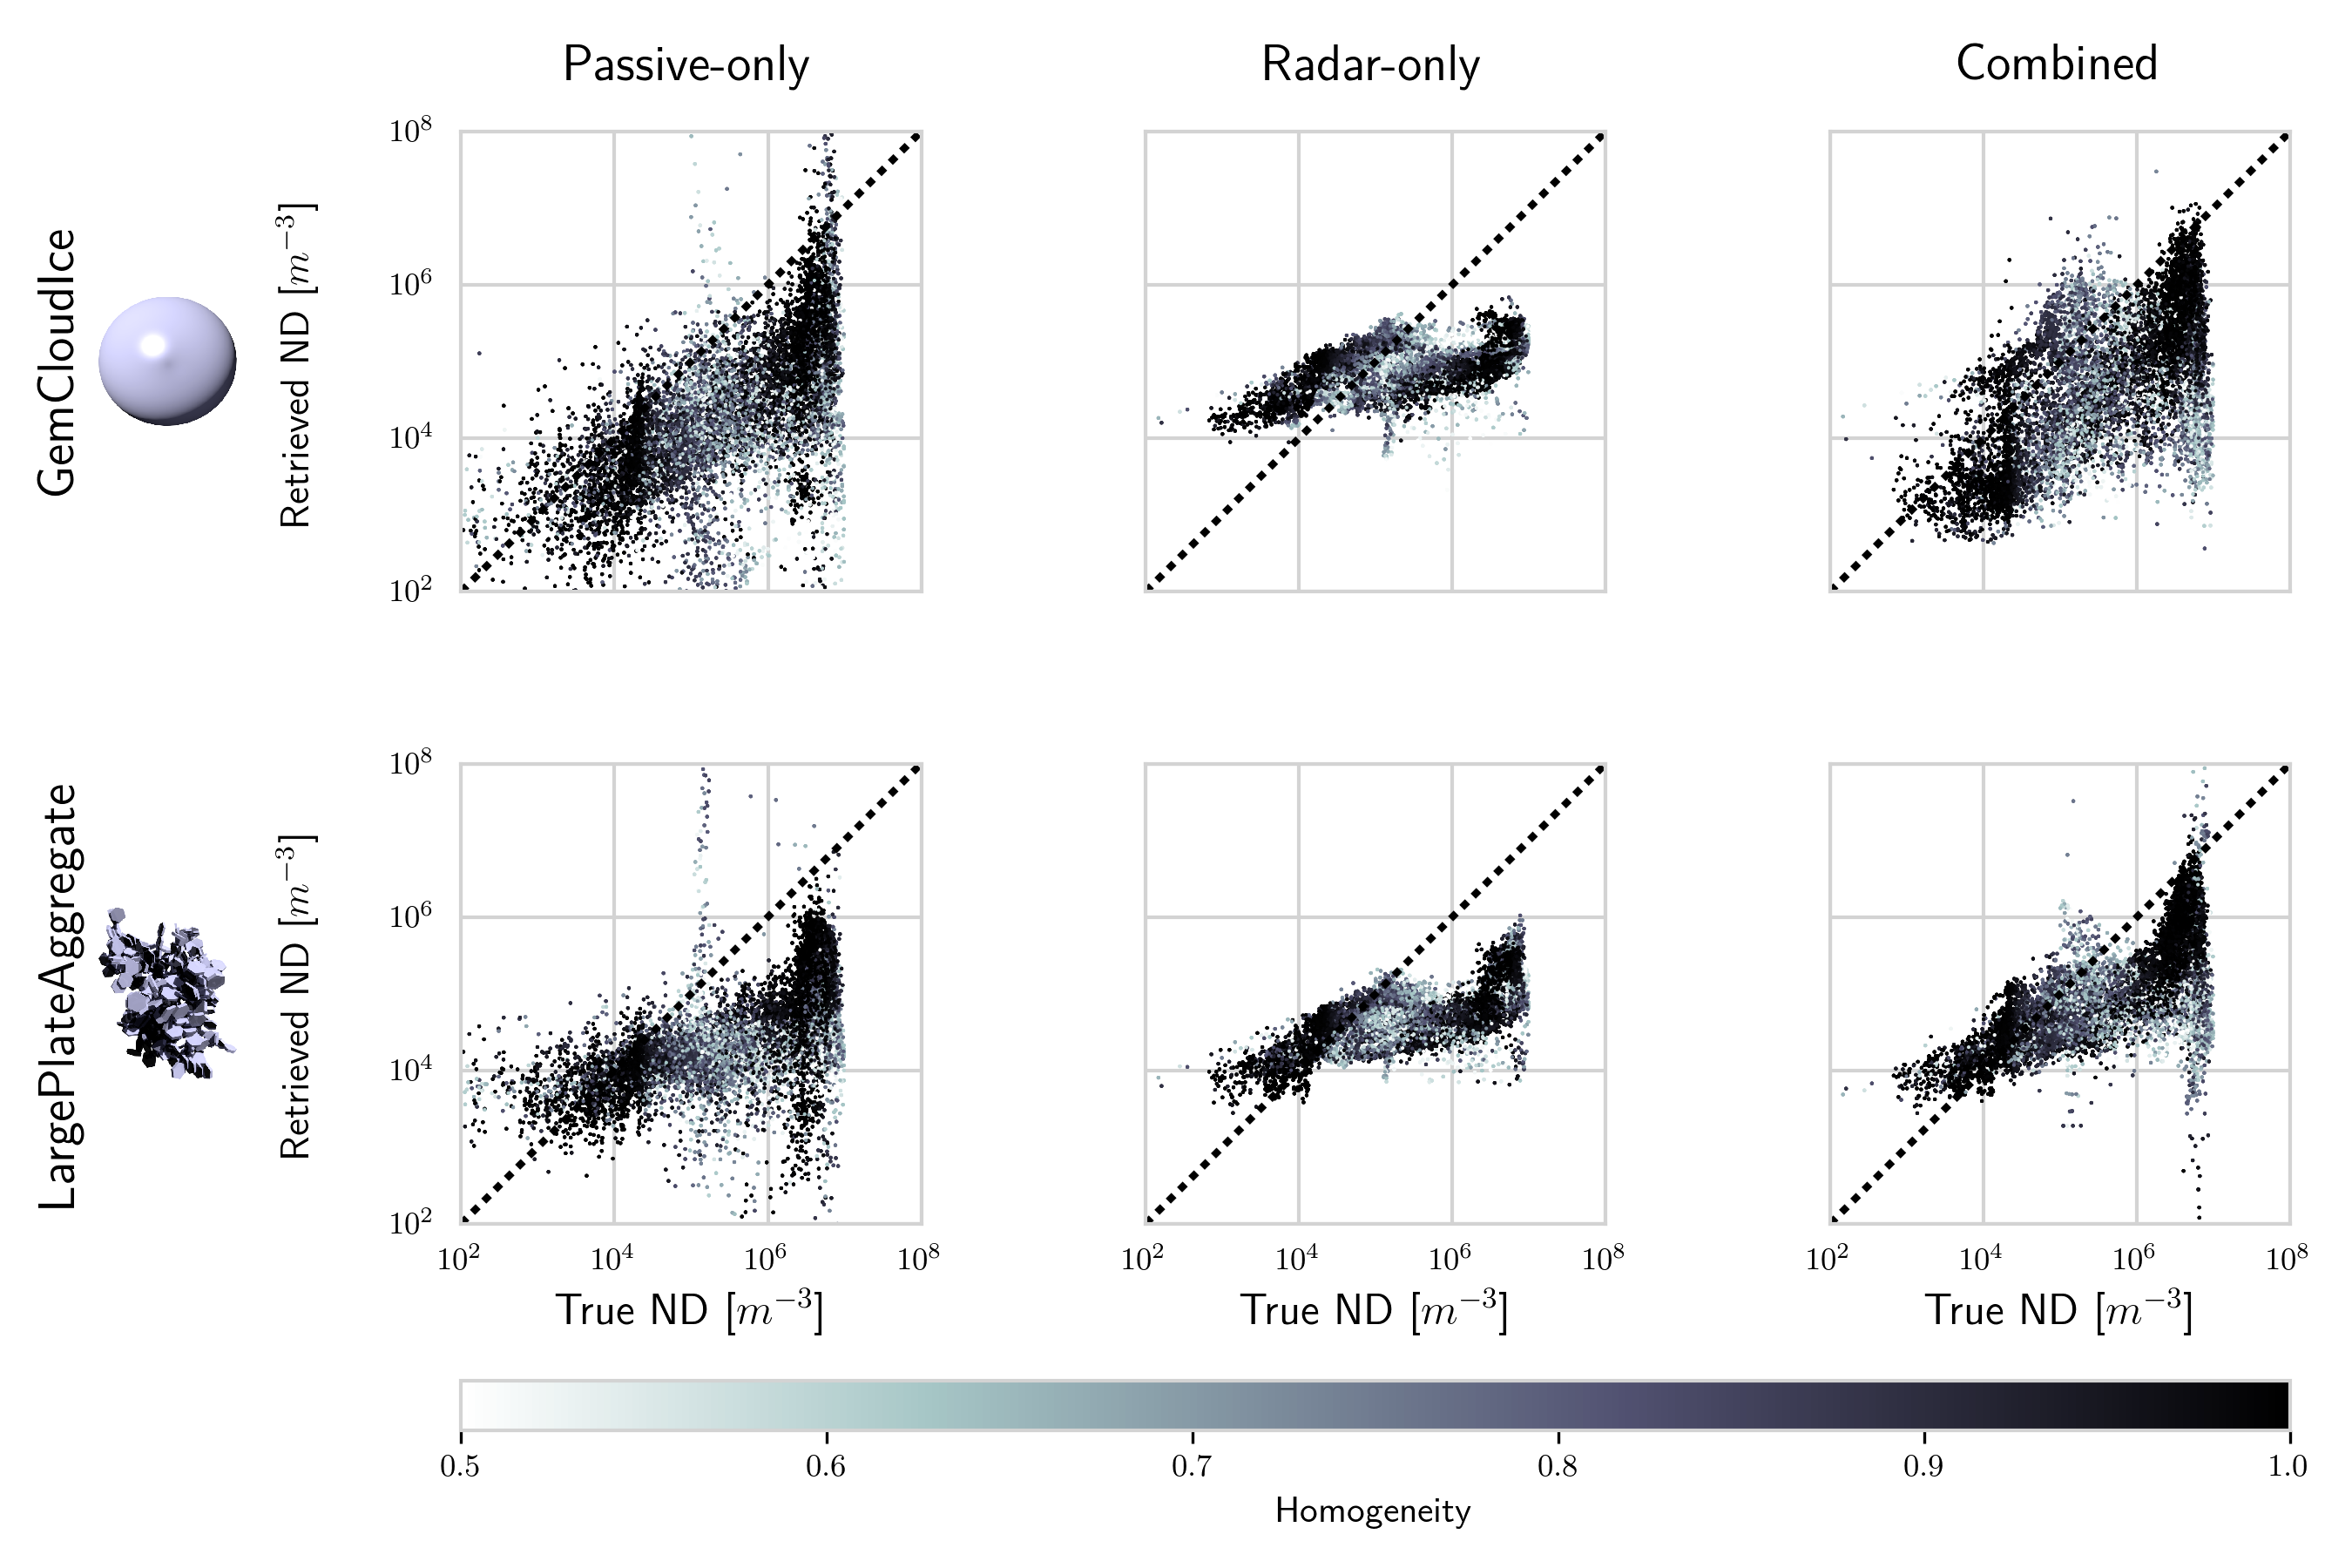
\includegraphics[width = 0.7\textwidth]{../plots/results_nd_scatter_a}
\caption{Scatter plots of the retrieved particle number densities at grid points
  with reference mass density larger than $10^{-5}\ \unit{kg/m^3}$. Rows show
  the results for the different particle models used in the retrieval while
  column display the results for the different retrieval methods. The marker
  color encodes the homogeneity of the corresponding ice mass computed as the
  ratio of the maximum mass density of any of the frozen hydrometeor species and
  the total ice mass density.}
\label{fig:results_nd_scatter_a}
\end{figure}

\subsubsection{Impact of assumed ice particle shape}

To allow the comparison of the retrieval performance for all tested retrievals
and particle shapes, the logarithmic error for the retrieved IWC and IWP are
displayed in Fig.~\ref{fig:boxes}. Considering first the results of the IWC
retrieval, shown in Panel~(a) and (b), the plots confirm the findings from the
analysis above: The combined retrieval generally yields the smallest retrieval
errors. Especially for the second test scene, where snow constitutes the major
part of the ice mass, the radar only retrieval produces significant systematic
errors, that are corrected by the combined retrieval.

At the same time, however, the combined retrieval exhibits a fairly strong
dependence on the applied particle model. This becomes apparent particularly in
the errors of the retrieved IWP, shown in Panel~(c) and (d), in which the
systematic deviations observed in the IWC retrieval are enhanced. In particular
the GemCloudIce and GemSnow particle models stand out as yielding the largest
systematic deviations.


\begin{figure}[!h]
\centering
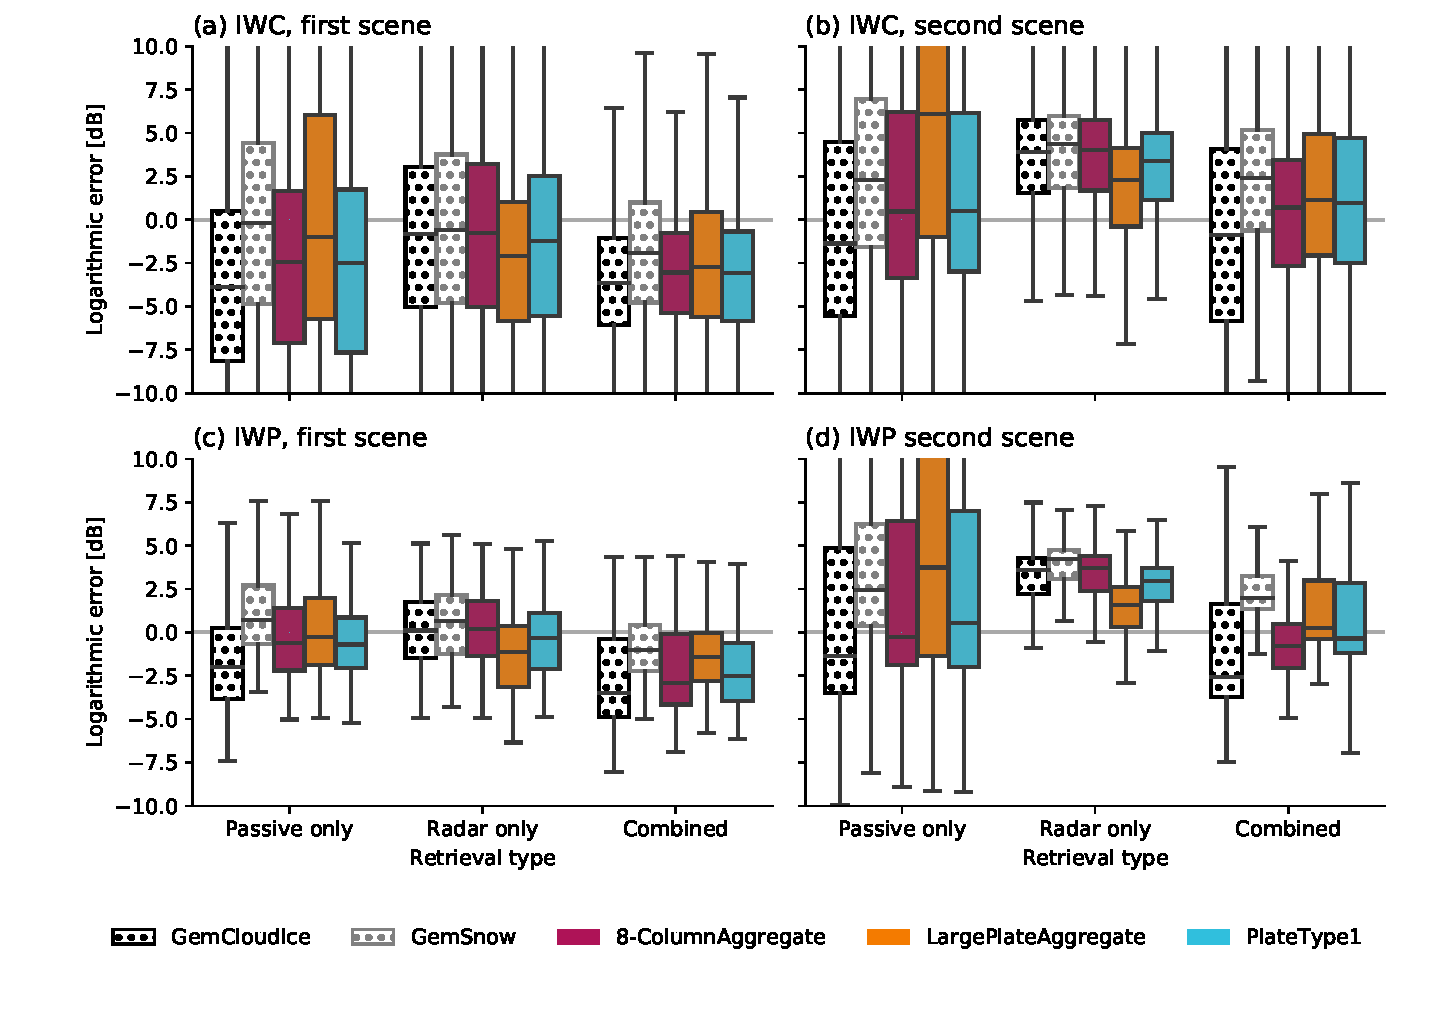
\includegraphics[width = 0.8\textwidth]{../plots/results_box}
\caption{Distributions of the logarithmic retrieval error in IWC and IWP for all tested retrieval
  methods and particle shapes displayed as box plots.}
\label{fig:boxes}
\end{figure}


To further investigate the effect the that the assumed ice particle shape has
on the retrieval results, the mass density relations for the tested particle
models are displayed in Panel~(a) of Fig.~\ref{fig:costs}. As can be seen from
this plot, the mass size relationship of the GemCloudIce particle clearly
stands out as being more dense than the others. On the contrary, the other
particles have quite similar mass size relationships. This may explain why
the GemCloudIce particle model does not work well for snow in the combined
retrievals, explaining the observed deviations in the retrieved mass densities.

Also displayed in Fig~\ref{fig:costs} (panel (b) and (c)) are the final OEM
costs of the combined retrieval that were obtained with the different particle
models for both test scenes. Since the particle shape has considerable effect on
sub-millimeter observations \citep{ekelund19}, one could hope that the retrieval results can be
used to infer the prevailing ice particle shape within the cloud based on the
quality of the fit of the forward model achieved during the retrieval.

Unfortunately, such clear conclusions cannot be drawn from the results. In the
first test scene, the best fit is obtained by the GemSnow, GemCloudIce and the
LargePlateAggregate particle models, although the GemSnow and GemCloudIce models
quite clearly yield the worst retrieval performance. For the second scene,
similar results are observed. Here, the GemSnow particle consistently gives the
lowest OEM cost but comparison with Fig~\ref{fig:boxes} clearly shows that it
doesn't yield the best retrieval performance.

\begin{figure}[!h]
\centering
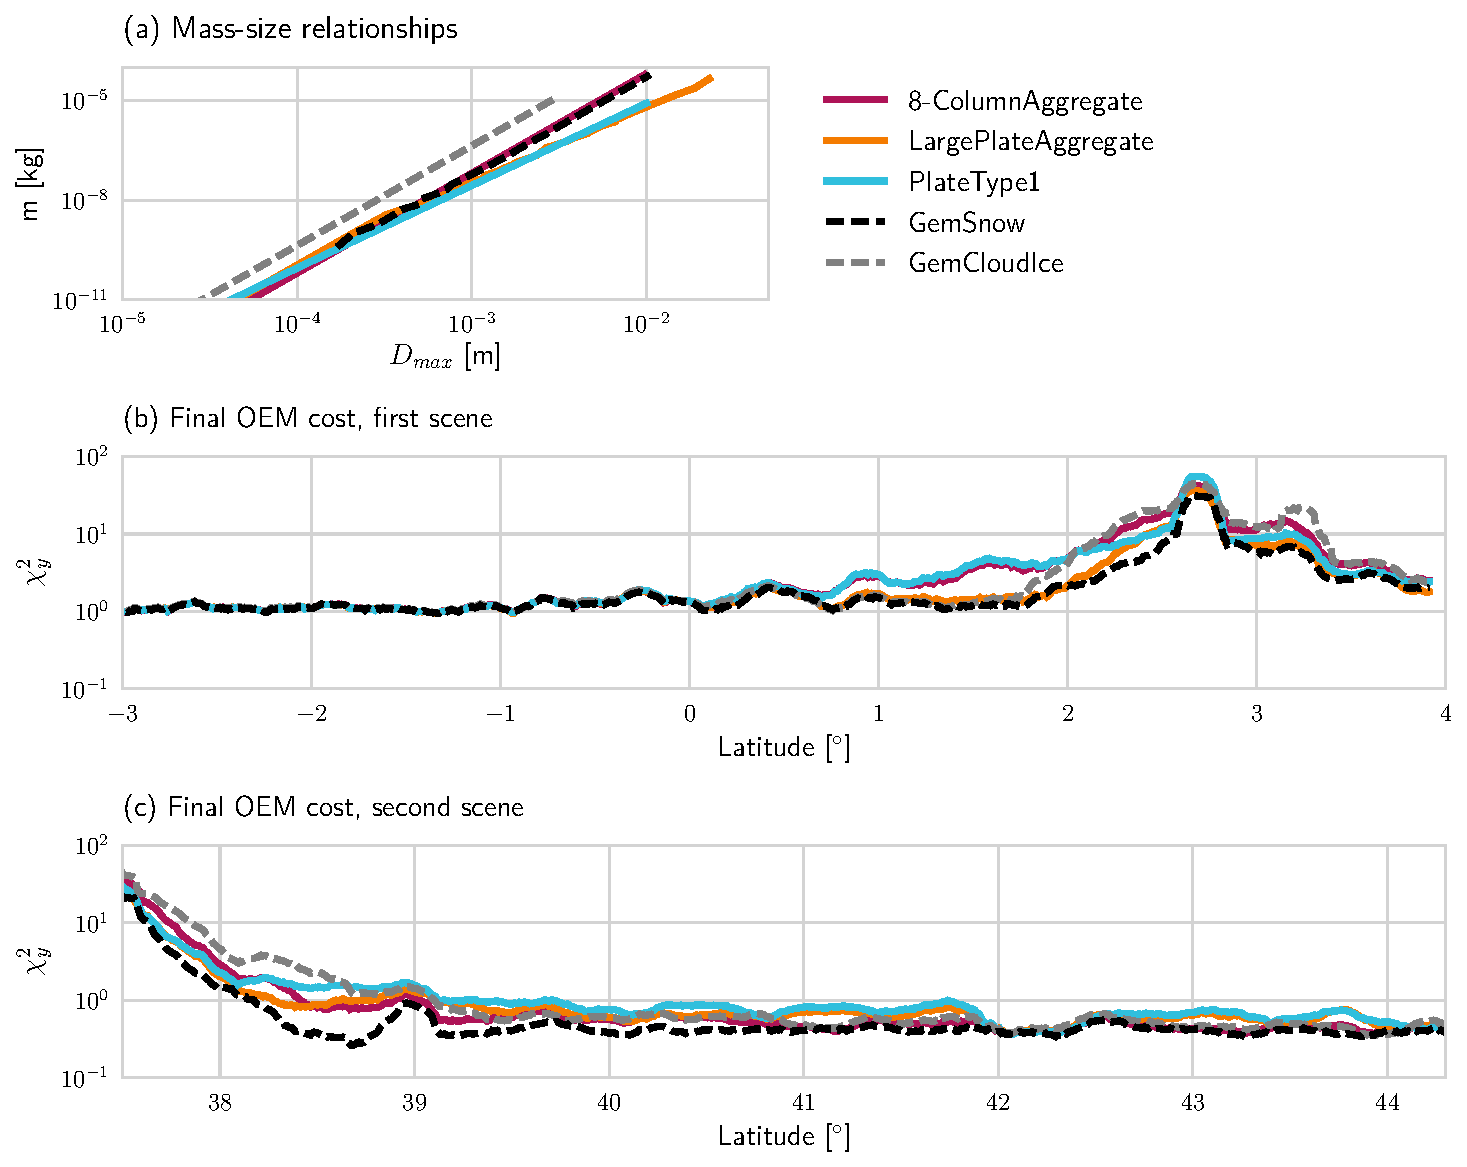
\includegraphics[width = 0.8\textwidth]{../plots/costs}
\caption{Mass-size relations (Panel (a)) and final OEM cost for the two test scenes
  (Panel (b) and (c)). The final cost curves where smoothed using a running average filter
of a width of 20 profiles.}
\label{fig:costs}
\end{figure}


\subsubsection{Humidity and cloud water}

The developed passive and combined retrieval algorithms also retrieve profiles
of humidity and liquid cloud mass density. For relative humidity, both
retrievals show sensitivity but no improvement could be observed in the results
of the combined retrieval compared to the passive-only retrieval. Moreover, no
suitable retrieval setup was found that yields satisfactory performance within
the scope of this study. We do not consider our results representative of what
could be achieved with the observational approach and thus do not include them
here.

Nonetheless, we provide results from the liquid cloud retrieval since these show
another interesting synergy of the radar and passive microwave observations.
Panel~(a) in Fig.~\ref{fig:results_cw_b} displays the reference and retrieved
column-integrated liquid cloud mass density (LWP). Although both retrievals
systematically underestimate the LWP, the underestimation is clearly reduced in
the combined retrieval.

Panel (b), (c) and (d) of Fig.~\ref{fig:results_cw_b} display contours of the
retrieved mass density field of liquid cloud drawn on top of the retrieved
frozen hydrometeor mass density field for the passive-only and the combined
retrieval. These results show clearly that the combined retrieval is able to
detect and retrieve liquid clouds even when they overlap with ice clouds.
Although some sensitivity of the retrieval to liquid clouds can be observed also
in the passive retrieval, the cloud is put at the wrong altitude and its mass
density is greatly underestimated. This indicates that the radar reflectivity
profile contains useful information for the retrieval to better locate cloud
water in the atmospheric column.

\begin{figure}
\centering
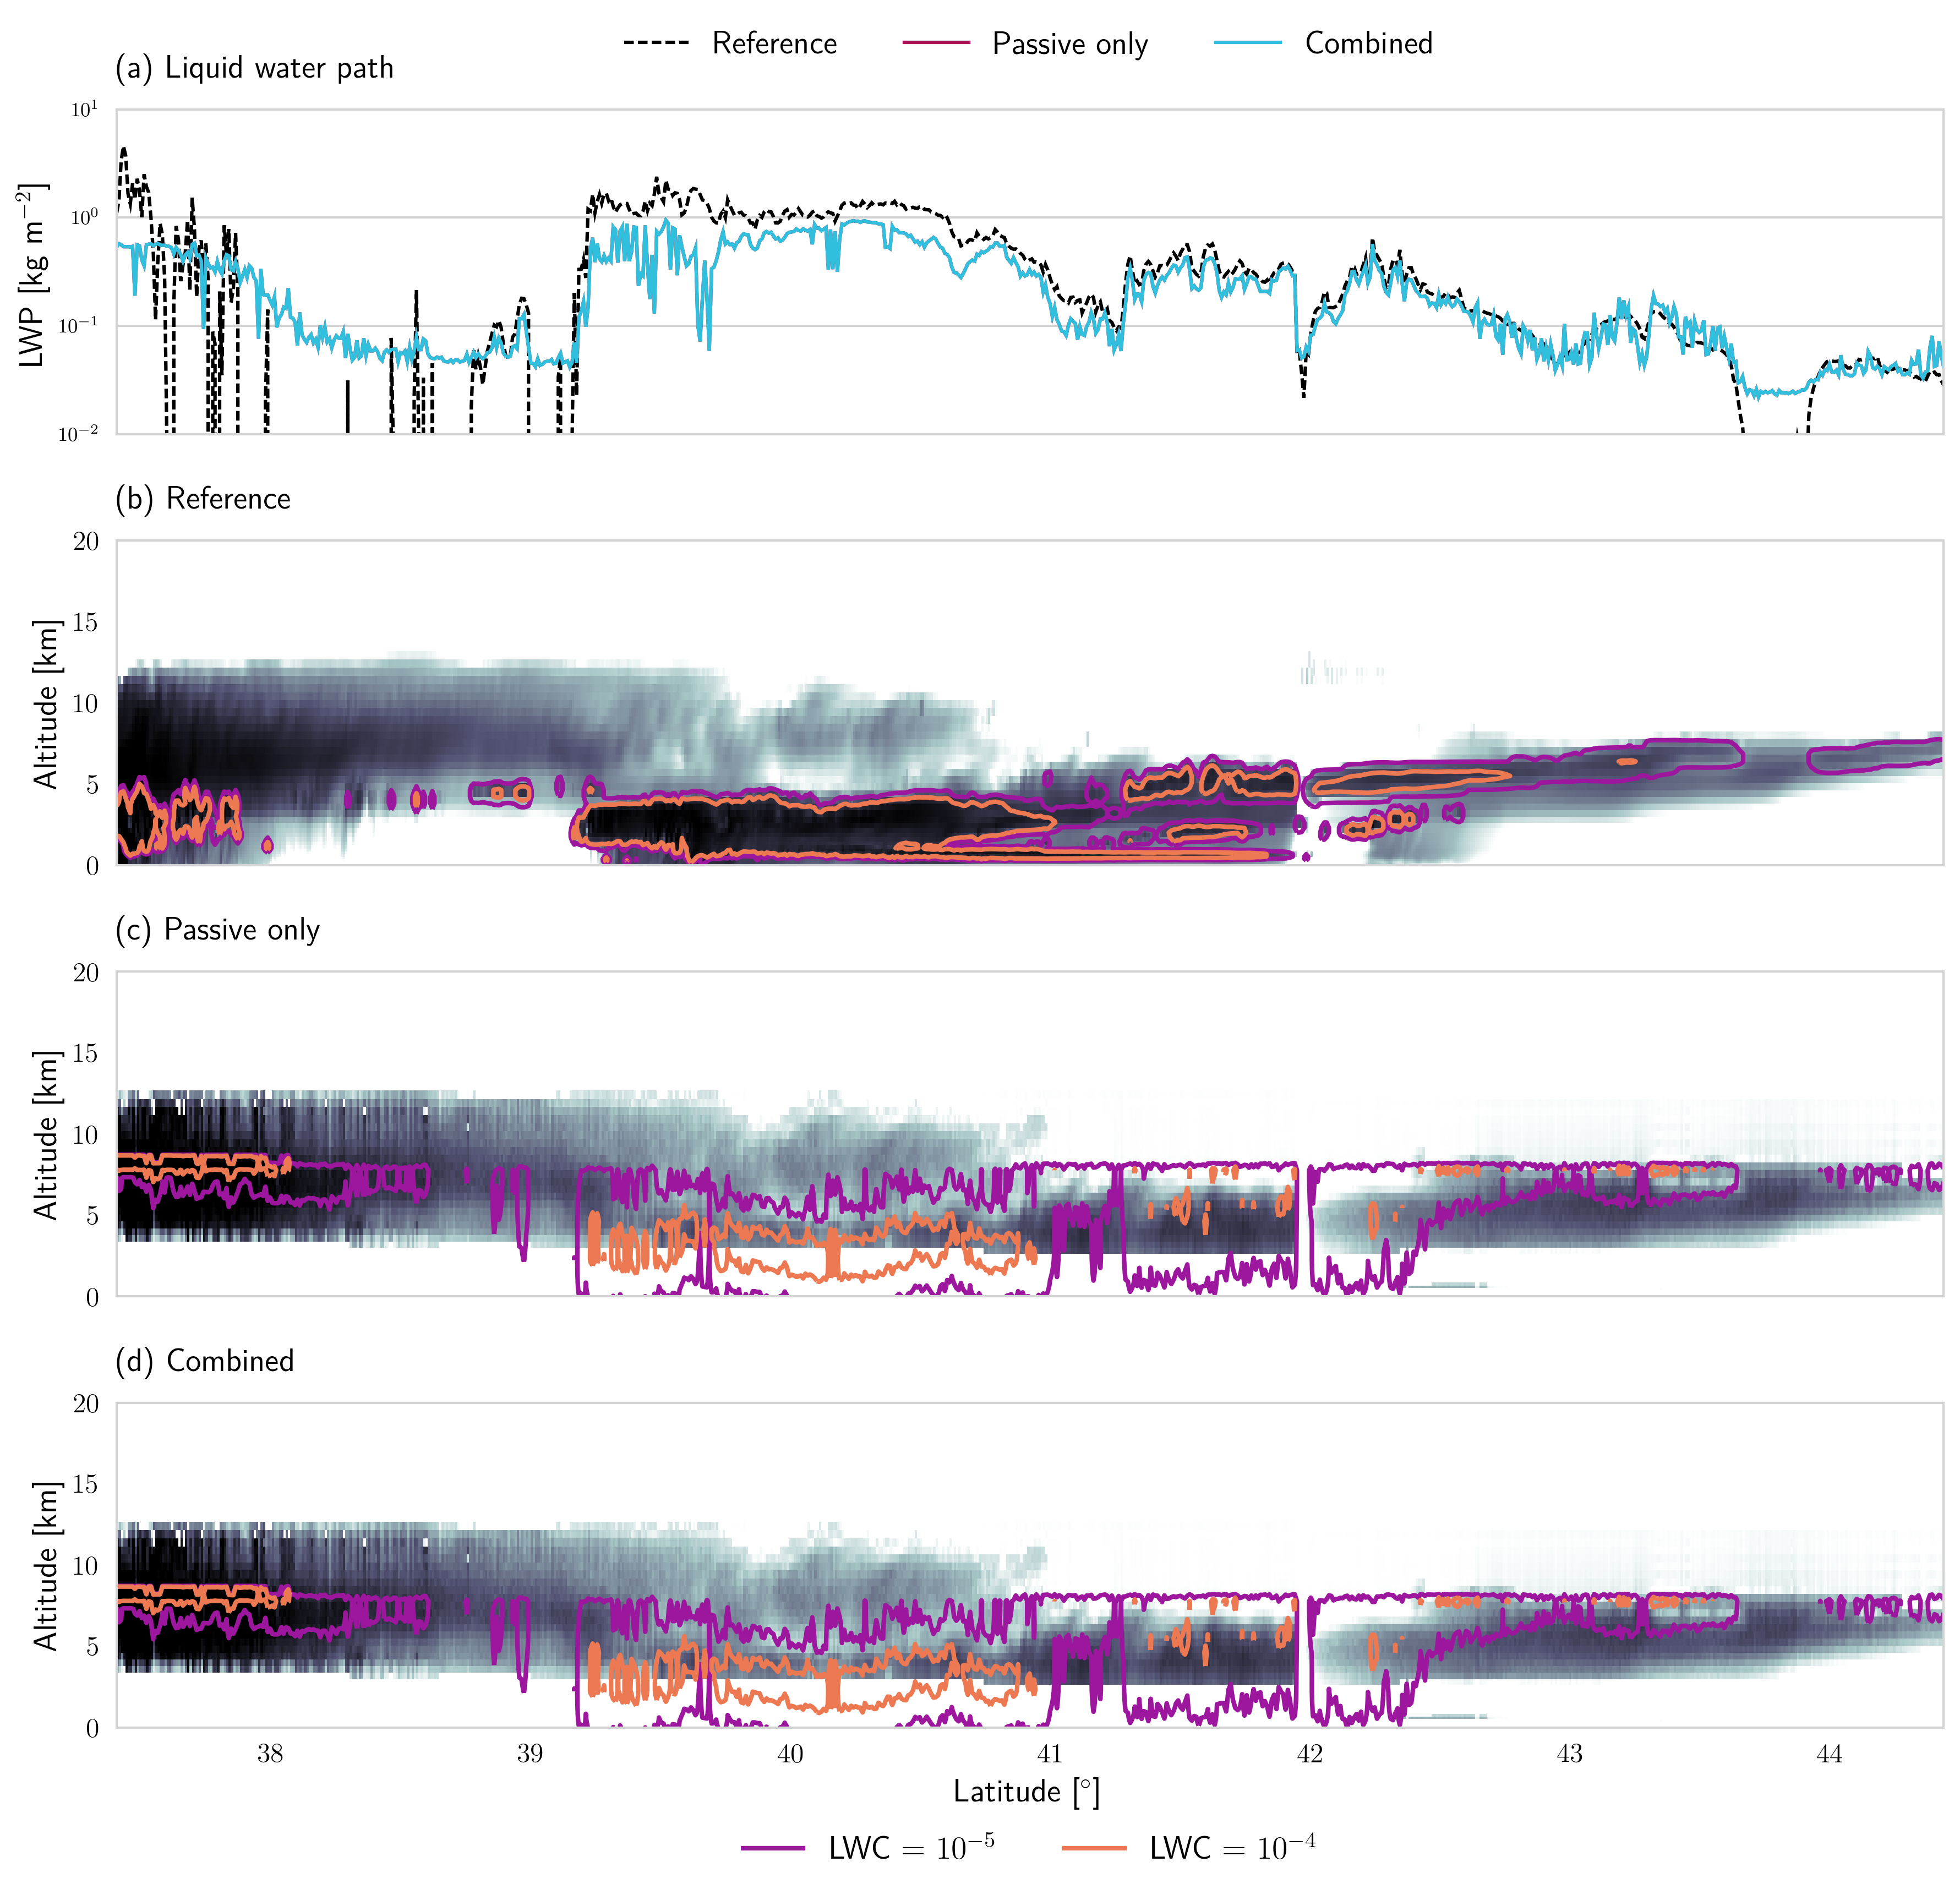
\includegraphics[width = \textwidth]{../plots/results_cw_b_LargePlateAggregate}
\caption{Contours of the cloud water mass density field drawn on top of the retrieved
  frozen hydrometeor mass density field. The results shown were obtained using the
  LargePlateAggregate particle model.}
\label{fig:results_cw_b}
\end{figure}


\section{Discussion}
\label{sec:discussion}

The principal aim of this study was to investigate the synergies between radar
and passive sub-millimeter observations. To this end, a simplified numerical
experiment has been presented, that qualitatively demonstrates the
complementarity of the information contained in the radar and the sub-millimeter
observations. Furthermore, a combined retrieval algorithm has been developed to
demonstrate the feasibility of the synergistic retrievals and further explore
their potential and current limitations.

\subsection{Fundamental synergies}

The experiment presented in the first part of this study aimed to establish the
fundamental synergies of the active and passive microwave observations. It
compared the cloud signals observed by a radar, a millimeter-wave radiometer and
a sub-millimeter-wave radiometer. The results show that the combined
observations can constrain the horizontal as well as the vertical scaling of the
particle size distribution. However, the complementary information content
between the active and passive observations depends on both the properties of
the observed cloud and the frequency of the observations. For the lower
frequencies considered in this study, i.e. the highest channels of the MWI
radiometer, the regions where both observations provide complementary
information on the particle size distribution of the cloud are limited to very
high mass densities and particle sizes. It should be noted, however, that since
the radar simulations neglect multiple scattering, the results are likely
less accurate in this region of the cloud-parameter space.

As the passive observing frequency increases, the regions of complementary
information content extend down to smaller particle sizes and cloud mass
density. Especially the highest-frequency channels of the ICI radiometer can
therefore be expected to provide additional information on the particle size
distribution of ice clouds.

\subsection{Combined cloud retrieval}

In the second part of the study, we have presented results from a combined,
variational cloud retrieval applied to synthetic observations from two test
scenes from a high-resolution atmosphere model. The results of the combined
retrieval were compared to that of a passive- and a radar-only version of the
retrieval algorithm. The simulated observations neglected potential errors
caused by different or non-overlapping antenna beams as well as inhomgeneity of
the atmosphere across the beams. A source of forward model error was included in
the simulated observations by performing them applying the full microphysics
scheme from the GEM model. This allowed to assess of the effect of cloud
composition as well the simplified microphysics used in the retrieval forward
model on the results.

Of the three considered retrieval implementations, the passive-only retrieval
clearly yields the worst performance for the retrieval of mass-density profiles.
It should be noted, however, that the passive only retrieval presented here has
not been optimized to its full potential and should therefore not be taken as
representative for the performance of the MWI and ICI radiometers. To ensure a
fair comparison, the passive only retrieval uses very similar a priori
assumptions as the other two retrievals, which in the presented case provide
only very limited information on the vertical structure of the cloud. As other
studies have shown, the passive observations do provide information on the
vertical distribution of ice in the atmospheric column \citep{wang17,
  grutzun18}, but the information content is limited to a few degrees of
freedom. It is therefore unlikely, that the vertical resolution of the
passive-only retrieval can be improved drastically without further constraining
it a priori, for example through an observation database in an empirical
retrieval.

As expected, the radar-only retrieval provides much better profile retrievals
than the passive-only version. However, the results exhibit systematic
deviations from the reference mass densities. Closer inspection revealed that
these are caused by an underestimation of the mass density of cloud ice and a
simultaneous overestimation of the mass density of snow. This indicates that the
a priori assumptions used in the retrieval do not fit the way ice and snow are
represented in the model, which causes the systematic deviations in the
retrieved mass densities. This observation is confirmed by the number density
fields retrieved from the radar-only retrieval. These are too low at regions
consisting mostly of cloud ice and too high in regions consisting of mostly
snow. Since the radar-only number density retrieval does not show signs of
sensitivity to the particle number density in the cloud, the reason for this
retrieval error are likely the a priori-assumed microphysical properties of the
hydrometeors.

The a priori assumptions that were used in this study were similar but not
identical to what is used in the DARDAR retrievals. Also here it should be
noted, that the presented results should not be taken to be representative for
the DARDAR product. Rather than this, the DARDAR a priori settings were chosen
since they represent well established and validated assumptions for ice cloud
retrievals and therefore should provide a reasonable starting point for the
development of a combined cloud retrieval. The fact that the a priori
assumptions used in the DARDAR retrieval do not agree with the microphysical
properties of ice and snow in the model, does not say much about the general
validity of these assumptions.

Despite the fact that the combined retrieval produced certain artefacts in the
results, our analysis showed that it was, at least for most of the tested
particle models, able to correct the systematic deviations in the retrieved mass
density field, that were observed in the radar-only retrieval. The benefit of
the combined observations was even more pronounced in the retrieved number
density fields. Here, neither the passive- or radar-only retrieval showed any
skill in retrieving the particle number concentrations. The combined retrieval,
however, was able to reproduce the general structure of the number concentration
fields in regions where the cloud composition was homogeneous. This clearly
shows that the joint observations constrain the cloud microphysics better than
the passive or radar observations alone.

Although the presented combined observations can improve the retrieval of frozen
hydrometeors, its performance can even degrade if an unrealistic particle habit
is used. These systematic errors were even more pronounced in the retrieved IWP.
Moreover, the combined retrieval displayed a stronger dependence of the
retrieval error on the assumed particle shape than the radar-only retrieval did.
The increased sensitivity of the combined retrieval to the microphysical
properties of the cloud thus increases the importance of a realistic particle
model.

A further note on the nature of the used particle models is in order here: The
GemCloudIce and GemSnow particle models are simple models, that use a single
shape that is scaled in size. Contrary to this, the three other models consist
of pristine crystals up to a certain size and of aggregates for larger sizes.
Generally, these habit models yield more accurate results than the simple models
confirming the usefulness of this approach. However, it was not possible to
deduce a clear relation between the mass-size relation of the particle model to
the retrieval performance. Although a likely explanation for the bad performance
of the GemCloudIce particle model is its unrealistic density, the mass-size
relation alone cannot explain why the LargePlateAggregate performs best as
particle model.

[Not to sure if previous paragraph is correct but felt that this should be mentioned
  here]

Furthermore, it has been briefly investigated whether the final OEM cost
function can provide information on the suitability of the chosen particle
model. Unfortunately, this was not the case. The underlying question aimed to
address with this experiment was whether the combined observations can constrain
the particle shape or whether instead a good fit to the observations can be
obtained regardless of the applied particle model. In the experiment no evidence
of a relation between the final OEM cost and the retrieval performance were
observed. From this, however, it can not be concluded that the combined
observations cannot constrain the ice particle shape. An explanation for the
observed lack of a shape signal in the OEM cost are for example that the applied
particle model or PSD are still too simple to describe a mixture of ice species
in the atmospheric column.

As an outlook, we have also included results of a liquid cloud retrieval, that
clearly shows the capability of the combined retrieval to distinguish liquid
clouds from ice clouds and retrieve profiles of liquid cloud mass densities.
Since the passive-only retrieval was unable to locate the cloud at the correct
altitude in the atmosphere, this constitutes an additional synergy between the
active and passive observations. Although no satisfactory results were obtained
from the water vapor retrieval, the retrieval results still indicate sensitivity
of this setup for retrieving atmospheric humidity. The full exploration of the
potential of the combined observations for liquid cloud and water vapor is out
of the scope of this study and is left to future investigation.

The combined retrieval implementation showed robust performance on fairly
distinct and complex cloud scenes. Despite this, both scenes that were
considered here contained parts where the OEM minimization did not find a state that
results in a good fit to the observations. In contrast to that, the radar-only
retrieval did converge well in most regions where the final cost of the combined
retrieval remained high. This points towards the existence of additional
information in the combined observations, that the retrieval method is not able
to disentangle. This raises the question of the suitability of the OEM method
applied here. The combined retrieval violates the two fundamental assumptions of
the OEM method: The forward model is non-linear and the assumed Gaussian a
priori assumptions do not describe reality very well. In addition to that, the
current implementation of the retrieval is computationally very expensive. For
further development of the combined retrieval concept it may therefore be
advisable to revisit the applied retrieval method in search for a potentially
more suitable alternative.

Finally, it is important to consider the limitations of this study. Its primary
limitation is certainly the restriction to the model scenes for the testing of
the retrieval. In addition to that, the forward simulations used to generate the
synthetic observations do not consider beam filling issues, assume a slightly
unrealistic viewing geometry and neglect multiple scattering in the radar
simulations. It is therefore important to understand the results presented here
in their qualitative sense rather than providing realistic performance
characteristics of the considered retrieval methods.

\conclusions  %% \conclusions[modified heading if necessary]
\label{sec:conclusions}

From the results presented above it can be concluded that complementary
information contained in radar and passive microwave radiometer observations can
be used to improve the retrieval of distributions of frozen hydrometeors in the
atmosphere. Altough dependent on the passive observing frequency and the
properties of the cloud itself, the combined observations can constrain both the
vertical and horizontal scaling of the PSD, which is not possible from radar
observations alone. For traditional microwave frequencies below $187
\ \unit{GHz}$ this capability, is limited to thick clouds consisting of large
and likely precipitating particles. The higher-frequency channels of the
upcoming ICI radiometer, however, when combined with a cloud radar will allow to
determine both scaling parameters even for thinner ice clouds made up of smaller
particles. In the conducted retrieval experiments, this allowed the combined
retrieval to distinguish the microphysical properties of cloud ice and snow and
thus reduce systematic errors observed in the radar-only IWC retrieval. In
addition to this, the combined retrieval displayed clear signs of sensitivity to
the particle number density field, which was not the case for the radar-only
retrieval.

At the same time, the combined retrieval exhibited a strong dependence of the
retrieval performance on the applied particle model. In particular for one of
the models a significant increase in the systematic retrieval error could be
observed compared to the radar-only retrieval. While the bad performance of this
specific particle model could be understood on the base of its unrealistically
high density, no clear explanation for performance differences of the other
particle models could be found. Furthermore, no relation between the OEM cost
and the aptness of the particle model could be established. Thus, to fully
exploit the potential of the combined retrievals further work is required to
understand the relation between properties of the ice particle model and the
impact of the model on the retrieval results. At the same time, this sensitivity
to the particle model opens up the possibility of using the combined retrievals
as a tool to test particle models by combining observations from field campaigns
with in-situ data.

In addition to that, our results also point towards an additional synergy
between the active and passive observations: The detection and retrieval of
liquid clouds. Although, the passive-only retrieval also showed sensitivity to
liquid clouds, the addition of the radar signal clearly improved the
localization in the atmospheric column and with that also LWP retrieval.

The results presented in this study clearly demonstrate the feasibility and
potential of combined retrievals of frozen hydrometeors using active and passive
microwave observations. The unique capability of the combined microwave
observations to better constrain cloud microphysics even inside thick clouds
could help to reduce remaining uncertainties in observations of ice the
atmosphere. As observational concept, such combined observations should
therefore be interesting for future field campaigns or space missions.


%% The following commands are for the statements about the availability of data sets and/or software code corresponding to the manuscript.
%% It is strongly recommended to make use of these sections in case data sets and/or software code have been part of your research the article is based on.

\codeavailability{All code used to produce the results in this study is available through a public repository \citep{ccrf}.} %% use this section when having only software code available


\dataavailability{} %% use this section when having only data sets available



\appendix
\section{}    %% Appendix A

\subsection{}     %% Appendix A1, A2, etc.


\noappendix       %% use this to mark the end of the appendix section

%% Regarding figures and tables in appendices, the following two options are possible depending on your general handling of figures and tables in the manuscript environment:

%% Option 1: If you sorted all figures and tables into the sections of the text, please also sort the appendix figures and appendix tables into the respective appendix sections.
%% They will be correctly named automatically.

%% Option 2: If you put all figures after the reference list, please insert appendix tables and figures after the normal tables and figures.
%% To rename them correctly to A1, A2, etc., please add the following commands in front of them:

\appendixfigures  %% needs to be added in front of appendix figures

\appendixtables   %% needs to be added in front of appendix tables

%% Please add \clearpage between each table and/or figure. Further guidelines on figures and tables can be found below.



\authorcontribution{Simon Pfreundschuh has implemented the retrieval, performed the data analysis and written
  the manuscript. Patrick Eriksson and Richard Larsson have contributed code to the ARTS radiative transfer
  model that was required to perform the presented calculations. Stefan A. Buehler, Patrick Eriksson, Manfred
  Brath and Simon Pfreundschuh have collaborated on the study that lead to the results presented here. David Duncan
and Robin Ekelund have contributed to the conceptualization of the study through comments and advice.} %% this section is mandatory for the journals ACP and GMD. For all other journals it is strongly recommended to make use of this section

\competinginterests{No competing interests are present} %% this section is mandatory even if you declare that no competing interests are present

\begin{acknowledgements}
TEXT
\end{acknowledgements}




%% REFERENCES

%% The reference list is compiled as follows:


%% Since the Copernicus LaTeX package includes the BibTeX style file copernicus.bst,
%% authors experienced with BibTeX only have to include the following two lines:

\bibliographystyle{copernicus}
\bibliography{references}
%%
%% URLs and DOIs can be entered in your BibTeX file as:
%%
%% URL = {http://www.xyz.org/~jones/idx_g.htm}
%% DOI = {10.5194/xyz}


%% LITERATURE CITATIONS
%%
%% command                        & example result
%% \citet{jones90}|               & Jones et al. (1990)
%% \citep{jones90}|               & (Jones et al., 1990)
%% \citep{jones90,jones93}|       & (Jones et al., 1990, 1993)
%% \citep[p.~32]{jones90}|        & (Jones et al., 1990, p.~32)
%% \citep[e.g.,][]{jones90}|      & (e.g., Jones et al., 1990)
%% \citep[e.g.,][p.~32]{jones90}| & (e.g., Jones et al., 1990, p.~32)
%% \citeauthor{jones90}|          & Jones et al.
%% \citeyear{jones90}|            & 1990



%% FIGURES

%% When figures and tables are placed at the end of the MS (article in one-column style), please add \clearpage
%% between bibliography and first table and/or figure as well as between each table and/or figure.


%% ONE-COLUMN FIGURES

%%f
%\begin{figure}[t]
%\includegraphics[width=8.3cm]{FILE NAME}
%\caption{TEXT}
%\end{figure}
%
%%% TWO-COLUMN FIGURES
%
%%f
%\begin{figure*}[t]
%\includegraphics[width=12cm]{FILE NAME}
%\caption{TEXT}
%\end{figure*}
%
%
%%% TABLES
%%%
%%% The different columns must be seperated with a & command and should
%%% end with \\ to identify the column brake.
%
%%% ONE-COLUMN TABLE
%
%%t
%\begin{table}[t]
%\caption{TEXT}
%\begin{tabular}{column = lcr}
%\tophline
%
%\middlehline
%
%\bottomhline
%\end{tabular}
%\belowtable{} % Table Footnotes
%\end{table}
%
%%% TWO-COLUMN TABLE
%
%%t
%\begin{table*}[t]
%\caption{TEXT}
%\begin{tabular}{column = lcr}
%\tophline
%
%\middlehline
%
%\bottomhline
%\end{tabular}
%\belowtable{} % Table Footnotes
%\end{table*}
%
%%% LANDSCAPE TABLE
%
%%t
%\begin{sidewaystable*}[t]
%\caption{TEXT}
%\begin{tabular}{column = lcr}
%\tophline
%
%\middlehline
%
%\bottomhline
%\end{tabular}
%\belowtable{} % Table Footnotes
%\end{sidewaystable*}
%
%
%%% MATHEMATICAL EXPRESSIONS
%
%%% All papers typeset by Copernicus Publications follow the math typesetting regulations
%%% given by the IUPAC Green Book (IUPAC: Quantities, Units and Symbols in Physical Chemistry,
%%% 2nd Edn., Blackwell Science, available at: http://old.iupac.org/publications/books/gbook/green_book_2ed.pdf, 1993).
%%%
%%% Physical quantities/variables are typeset in italic font (t for time, T for Temperature)
%%% Indices which are not defined are typeset in italic font (x, y, z, a, b, c)
%%% Items/objects which are defined are typeset in roman font (Car A, Car B)
%%% Descriptions/specifications which are defined by itself are typeset in roman font (abs, rel, ref, tot, net, ice)
%%% Abbreviations from 2 letters are typeset in roman font (RH, LAI)
%%% Vectors are identified in bold italic font using \vec{x}
%%% Matrices are identified in bold roman font
%%% Multiplication signs are typeset using the LaTeX commands \times (for vector products, grids, and exponential notations) or \cdot
%%% The character * should not be applied as mutliplication sign
%
%
%%% EQUATIONS
%
%%% Single-row equation
%
%\begin{equation}
%
%\end{equation}
%
%%% Multiline equation
%
%\begin{align}
%& 3 + 5 = 8\\
%& 3 + 5 = 8\\
%& 3 + 5 = 8
%\end{align}
%
%
%%% MATRICES
%
%\begin{matrix}
%x & y & z\\
%x & y & z\\
%x & y & z\\
%\end{matrix}
%
%
%%% ALGORITHM
%
%\begin{algorithm}
%\caption{...}
%\label{a1}
%\begin{algorithmic}
%...
%\end{algorithmic}
%\end{algorithm}
%
%
%%% CHEMICAL FORMULAS AND REACTIONS
%
%%% For formulas embedded in the text, please use \chem{}
%
%%% The reaction environment creates labels including the letter R, i.e. (R1), (R2), etc.
%
%\begin{reaction}
%%% \rightarrow should be used for normal (one-way) chemical reactions
%%% \rightleftharpoons should be used for equilibria
%%% \leftrightarrow should be used for resonance structures
%\end{reaction}
%
%
%%% PHYSICAL UNITS
%%%
%%% Please use \unit{} and apply the exponential notation


\end{document}
